\newcommand{\UseWhiteBackground}{1}  % Copy this to have a white document
\documentclass[]{scrarticle}
% \newcommand{\lang}{french}  % Copy this in a french document
% \newcommand{\UseWhiteBackground}{1}  % Copy this to have a white document

\usepackage[utf8]{inputenc}
\usepackage{standalone}
\usepackage{etoolbox}
\ifdef{\lang}{}{\newcommand{\lang}{english}}  % If no \lang command is defined, default to english
\usepackage[\lang]{babel}
\usepackage{amssymb,amsmath,amsthm,epsfig,eepic,epic,verbatim,moreverb,fancybox}
\usepackage{stmaryrd}  % for \llbracket and \rrbracket
\usepackage{wasysym}
% \usepackage{bbold}  % NO! DON"T USE IT. It add mathbb for integers but makes it ugly for letters.
\usepackage{dsfont}
% \usepackage{tocstyle}  % To change the table of contents (TOC) style, and that's what we do next
% \usetocstyle{nopagecolumn}  % One of classic, KOMAlike, nopagecolumn, allwithdot, noonewithdot, standard
\usepackage{tikz}
\usepackage{tikz-cd}
\usetikzlibrary{calc,math,decorations.markings,decorations.pathmorphing,arrows,shadows,shapes.geometric,shapes.multipart,patterns,automata,backgrounds}
\usepackage{rotating}  % To have large figures in lanscape with \begin{sidewaysfigure} ... \end{sidewaysfigure}
\usepackage{pdflscape}  % To change one page to landscape
\usepackage{multicol}  % For the \begin{multicol}{N} environement
\usepackage{wrapfig}   % For the \begin{wrapfig}{r|l}{4cm} environement that behave like html float
\usepackage{subcaption}  % To use the subfigure environement in figure environements
\usepackage{multirow}  % Use \multirow{N}{*}{text} to have text in N rows in a table
\usepackage{mathtools}  % For the \xSOMETHINGarrow that we can write on top and change length
\usepackage{xspace}  % To add a space in commands when the following is not pounctuation
\usepackage{todonotes}  % To add todos in the margin of a document with \todo. Also \listoftodos is nice !
\usepackage{graphicx}  % many operations like rotating text etc...
\usepackage{ifthen}
\usepackage{xifthen}
\usepackage{float}  % To have the [H] option for figure so that they don't float. Use only if really needed.
\usepackage{pdfpages}
\usepackage{tablefootnote}  % To have footnotes in tables, use \tablefootnote{...}
\usepackage{enumerate}  % To be able to change the numbering of enumerate environements with [i)] or [a.]...
\usepackage{enumitem}  % To manage the spacing of items and margins
\usepackage{forest}  % For automatic tikz layout
\usepackage[framemethod=tikz]{mdframed}  % Frame around theorems
\usepackage{thmtools}  % Fixes the issue with \autoref and shared counters for thm env. Probably lots of other things also...
\usepackage{listings}
% \usepackage{minted}
\usepackage{pbox}  % A variable width parbox
\usepackage{xcolor}

\definecolor{airforceblue}{rgb}{0.36, 0.54, 0.66}
\definecolor{awesome}{rgb}{1.0, 0.13, 0.32}
\definecolor{bondiblue}{rgb}{0.0, 0.58, 0.71}
\definecolor{atomictangerine}{rgb}{1.0, 0.6, 0.4}
\definecolor{ghostwhite}{rgb}{0.97, 0.97, 1.0}

% creamy background
\ifdef{\UseWhiteBackground}{  % White, default
    \definecolor{myBGcolor}{HTML}{FFFFFF}
    \definecolor{myTextcolor}{HTML}{000000}
    \definecolor{linkColor}{HTML}{044F67}

    % \colorlet{linkColor}{orange!60!blue}
    \colorlet{myRed}{awesome!10!myBGcolor}
    \colorlet{myGreen}{airforceblue!15!myBGcolor}
}{  % Cream
    \definecolor{myBGcolor}{HTML}{E6E0C6}
    \definecolor{myTextcolor}{HTML}{2F251C}
    \colorlet{linkColor}{orange!70!blue}

    \pagecolor{myBGcolor}
    \color{myTextcolor}

    \colorlet{myRed}{awesome!10!myBGcolor}
    \colorlet{myGreen}{green!10!myBGcolor}
}


\usepackage{hyperref}  % Always include it last, as it overrides a lot of commands.
\hypersetup{
    % bookmarks=true,
    % pdfpagemode=FullScreen,  % Only for presentations
    pdfauthor={Diego Dorn},
    pdftitle={ok},
    colorlinks=true,
    allcolors=linkColor
    % linkcolor=blue,
    % urlcolor={winered},
    % filecolor={winered},
    % citecolor={winered},
    % allcolors={orange},
    % linktoc=all,
}

% \usepackage{cleveref}  % Needs to be after hyperref

\addto\extrasenglish{%
    \renewcommand{\subsectionautorefname}{Section}  % Change name of subsection in autoref to be more uniform
}


% Tool to translate commands
% The first argument is the english text, the second is in french
\newcommand{\ifenglish}[2]{\ifthenelse{\equal{\lang}{english}}{#1}{#2}}

% Frames
\mdfdefinestyle{theoremstyle}{%
roundcorner=0pt, % round corners, makes it friendlier
leftmargin=1pt, rightmargin=1pt, % this helps with box warnings
innerbottommargin=12pt,
hidealllines=true, % even friendlier
align=center, %
}

% Theorem environements
\theoremstyle{definition}   % Not in italics
\ifenglish{
    \newtheorem{theorem}{Theorem}[section]
    \newtheorem*{theorem*}{Theorem}
    \newtheorem{theoremx}{Theorem}
    \newtheorem{definition}[theorem]{Definition}
    \newtheorem{notation}[theorem]{Notation}
    \newtheorem{corollary}[theorem]{Corollary}
    \newtheorem{proposition}[theorem]{Proposition}
    \newtheorem*{proposition*}{Proposition}
    \newtheorem{lemma}[theorem]{Lemma}
    \newtheorem*{lemma*}{Lemma}
    \newtheorem*{remark}{Remark}
    \newtheorem*{claim}{Claim}
    \newtheorem*{example}{Example}
    \newtheorem*{examples}{Examples}
    \newtheorem*{exercise}{Exercise}
}{
    \newtheorem{theorem}{Théorème}[section]
    \newtheorem*{theorem*}{Théorème}
    \newtheorem{theoremx}{Théorème}
    \newtheorem{definition}[theorem]{Définition}
    \newtheorem{notation}[theorem]{Notation}
    \newtheorem{corollary}[theorem]{Corrolaire}
    \newtheorem{proposition}[theorem]{Proposition}
    \newtheorem{lemma}[theorem]{Lemme}
    \newtheorem*{remark}{Remarque}
    \newtheorem*{claim}{Assertion}
    \newtheorem*{example}{Exemple}
    \newtheorem*{examples}{Exemples}
    \newtheorem*{exercise}{Exercise}
}
\renewcommand{\thetheoremx}{\Alph{thmx}} % "letter-numbered" theorems


\surroundwithmdframed[style=theoremstyle,backgroundcolor=myRed]{theorem}
\surroundwithmdframed[style=theoremstyle,backgroundcolor=myRed]{theorem*}
\surroundwithmdframed[style=theoremstyle,backgroundcolor=myGreen]{definition}

%%%%%%%%%%%%%%%%%%%
%   Parenthesis   %
%%%%%%%%%%%%%%%%%%%

\newcommand{\parenthesis}[1]{\left(#1\right)}
\newcommand{\bigparenthesis}[1]{\big(#1\big)}
\newcommand{\Bigparenthesis}[1]{\Big(#1\Big)}
\newcommand{\Par}[2][]{
    \ifthenelse{\isempty{#1}}{%
        \mathopen{}\left(#2\right)\mathclose{}%
    }{\ifthenelse{#1 = 0}{
        (#2)%
    }{\ifthenelse{#1 = 1}{%
        \big(#2\big)%
    }{\ifthenelse{#1 = 2}{%
        \Big(#2\Big)%
    }{\ifthenelse{#1 = 3}{%
        \large(#2\large)%
    }{\ifthenelse{#1 = 4}{%
        \Large(#2\Large)%
    }{%
        \mathopen{}\left(#2\right)\mathclose{}%
    }}}}}}}
\newcommand{\Bra}[2][]{
    \ifthenelse{\isempty{#1}}{%
        \mathopen{}\left[#2\right]\mathclose{}%
    }{\ifthenelse{#1 = 0}{
        [#2]%
    }{\ifthenelse{#1 = 1}{%
        \big[#2\big]%
    }{\ifthenelse{#1 = 2}{%
        \Big[#2\Big]%
    }{\ifthenelse{#1 = 3}{%
        \large[#2\large]%
    }{\ifthenelse{#1 = 4}{%
        \Large[#2\Large]%
    }{%
        \mathopen{}\left[#2\right]\mathclose{}%
    }}}}}}}


\newcommand{\brackets}[1]{\left[#1\right]}

%%%%%%%%%%%%%%%%%%%
%    Operators    %
%%%%%%%%%%%%%%%%%%%

\DeclareMathOperator{\id}{id}
\DeclareMathOperator{\re}{Re}
\DeclareMathOperator{\Aut}{Aut}
\DeclareMathOperator{\Hom}{Hom}
\DeclareMathOperator{\Char}{char}
\DeclareMathOperator{\im}{Im}
\DeclareMathOperator{\dom}{dom}
\DeclareMathOperator{\cof}{cof}
\DeclareMathOperator{\Ob}{Ob}
\DeclareMathOperator{\Mor}{Mor}
\DeclareMathOperator{\rk}{rk}

\newcommand{\concat}{
  \mathord{
    \mathchoice
    {\raisebox{1ex}{\scalebox{.7}{$\frown$}}}
    {\raisebox{1ex}{\scalebox{.7}{$\frown$}}}
    {\raisebox{.7ex}{\scalebox{.5}{$\frown$}}}
    {\raisebox{.7ex}{\scalebox{.5}{$\frown$}}}
  }
}
\newcommand{\restr}[1]{\mathbin\upharpoonright_{#1}}
\newcommand{\compl}[1]{#1^\mathsf{c}}
\newcommand{\abs}[1]{\left| #1 \right|}
\newcommand{\bigabs}[1]{\big\lvert#1\big\rvert}
\newcommand{\parens}[1]{\left(#1\right)}
\newcommand{\norm}[1]{\left\| #1 \right\|}

%%%%%%%%%%%%%%%%%%%
%  Constructions  %
%%%%%%%%%%%%%%%%%%%

% Arrows
\newcommand{\xto}[1]{\xrightarrow{#1}}

% Structures
\newcommand{\verteqsign}{\rotatebox{90}{$\,=$}}
\newcommand{\verteq}[2]{\underset{\scriptstyle\overset{\mkern4mu\verteqsign}{#2}}{#1}}
\newcommand{\vertimplies}[2]{\underset{\scriptstyle\overset{\uparrow}{#2}}{#1}}
\newcommand{\func}[5]{
    \begin{array}{rccl}
            #1 : & #2 & \longrightarrow & #3 \\
                 & #4 & \longmapsto     & #5
    \end{array}
}
\newcommand{\ntimes}[2]{\underbrace{#1, \dots, #1}_{#2 \ttimes}}
% Reminder: for combinations / binomial coefficients, use \binom{n}{k}

% Set definitions
\newcommand{\set}[1]{\left\{ #1 \right\}}
\newcommand{\bigset}[1]{\big\{ #1 \big\}}
\newcommand{\setst}[2]{\left\{ #1 \, \middle| \, #2 \right\}}
\newcommand{\bigsetst}[2]{\big\{ #1 \, \big| \, #2 \big\}}

\newcommand{\funcset}[2]{{}^{#1}{#2}}
\newcommand{\angles}[1]{\left\langle #1 \right\rangle}
\newcommand{\brz}{B_r(z_0)}
\newcommand\quotient[2]{
    \mathchoice
        {% \displaystyle
            \text{\raise1ex\hbox{$#1$}\Big/\lower1ex\hbox{$#2$}}%
        }
        {% \textstyle
            #1\,/\,#2
        }
        {% \scriptstyle
            #1\,/\,#2
        }
        {% \scriptscriptstyle
            #1\,/\,#2
        }
}
\newcommand{\interior}[1]{\mathring{#1}}

%%%%%%%%%%%%%%%
%   Letters   %
%%%%%%%%%%%%%%%


% Greek alphabe
\renewcommand{\phi}{\ensuremath\varphi\xspace}
\renewcommand{\epsilon}{\ensuremath\varepsilon\xspace}
\renewcommand{\a}{\ensuremath\alpha\xspace}
\renewcommand{\d}{\ensuremath{\partial}\xspace}
\newcommand{\D}{\ensuremath\Delta\xspace}
\newcommand{\e}{\ensuremath\epsilon\xspace}
\newcommand{\g}{\ensuremath\gamma\xspace}
\newcommand{\y}{\g}  % I mistake them every other time
\newcommand{\p}{\phi\xspace}
\newcommand{\s}{\sigma\xspace}
\newcommand{\w}{\ensuremath\omega\xspace}

% Mathbb alphabet

\newcommand{\IB}{\ensuremath{\mathbb B}\xspace}
\newcommand{\C}{\ensuremath{\mathbb C}\xspace}
\newcommand{\ID}{\ensuremath{\mathbb D}\xspace}
\newcommand{\IE}{\ensuremath{\mathbb E}\xspace}
\newcommand{\F}{\ensuremath{\mathbb F}\xspace}
\newcommand{\IG}{\ensuremath{\mathbb G}\xspace}
\newcommand{\N}{\ensuremath{\mathbb N}\xspace}
\newcommand{\R}{\ensuremath{\mathbb R}\xspace}
\newcommand{\IP}{\ensuremath{\mathbb P}\xspace}
\newcommand{\IS}{\ensuremath{\mathbb S}\xspace}
\newcommand{\IT}{\ensuremath{\mathbb T}\xspace}
\newcommand{\Q}{\ensuremath{\mathbb Q}\xspace}
\newcommand{\Z}{\ensuremath{\mathbb Z}\xspace}
\newcommand{\ONE}{\text{\usefont{U}{bbold}{m}{n}1}}

% Fancy fonts
\newcommand{\Aa}{\ensuremath{\mathcal A}\xspace}
\newcommand{\Bb}{\ensuremath{\mathcal B}\xspace}
\newcommand{\Cc}{\ensuremath{\mathcal C}\xspace}
\newcommand{\Dd}{\ensuremath{\mathcal D}\xspace}
\newcommand{\Ee}{\ensuremath{\mathcal E}\xspace}
\newcommand{\Ff}{\ensuremath{\mathcal F}\xspace}
\newcommand{\Gg}{\ensuremath{\mathcal G}\xspace}
\newcommand{\Hh}{\ensuremath{\mathcal H}\xspace}
\newcommand{\Ii}{\ensuremath{\mathcal I}\xspace}
\newcommand{\Jj}{\ensuremath{\mathcal J}\xspace}
\newcommand{\Kk}{\ensuremath{\mathcal K}\xspace}
\newcommand{\Ll}{\ensuremath{\mathcal L}\xspace}
\newcommand{\Mm}{\ensuremath{\mathcal M}\xspace}
\newcommand{\Nn}{\ensuremath{\mathcal N}\xspace}
\newcommand{\Oo}{\ensuremath{\mathcal O}\xspace}
\newcommand{\Pp}{\ensuremath{\mathcal P}\xspace}
\newcommand{\Qq}{\ensuremath{\mathcal Q}\xspace}
\newcommand{\Rr}{\ensuremath{\mathcal R}\xspace}
\newcommand{\Ss}{\ensuremath{\mathcal S}\xspace}
\newcommand{\Tt}{\ensuremath{\mathcal T}\xspace}
\newcommand{\Uu}{\ensuremath{\mathcal U}\xspace}
\newcommand{\Vv}{\ensuremath{\mathcal V}\xspace}
\newcommand{\Ww}{\ensuremath{\mathcal W}\xspace}
\newcommand{\Xx}{\ensuremath{\mathcal X}\xspace}
\newcommand{\Yy}{\ensuremath{\mathcal Y}\xspace}
\newcommand{\Zz}{\ensuremath{\mathcal Z}\xspace}
\renewcommand{\O}[1]{\mathcal{O}\left(#1\right)}

% Others
\renewcommand{\emptyset}{\varnothing}


%%%%%%%%%%%%%%%%%%
%   New symbols  %
%%%%%%%%%%%%%%%%%%

\newcommand{\iddots}{{\cdot^{\cdot^\cdot}}}  % Three dots on the antidiagonal
\newcommand{\existsinf}{\exists^\infty}
\newcommand{\coloneq}{\mathrel{\resizebox{\widthof{$\mathord{=}$}}{\height}{ $\!\!\resizebox{1.2\width}{0.8\height}{\raisebox{0.23ex}{$\mathop{:}$}}\!\!=\!\!$ }}}  % Fancier :=

%%%%%%%%%%%%%%%%%%
%   Shorthands   %
%%%%%%%%%%%%%%%%%%

% Math text
\newcommand{\open}{\text{ open }}
\newcommand{\st}{\text{ \ifenglish{s.t}{t.q}. }}
\newcommand{\andd}{\text{ \ifenglish{and}{et} }}
\newcommand{\andquad}{\quad\andd\quad}
\newcommand{\et}{\text{ et }}
\newcommand{\ttimes}{\text{ times}}
\newcommand{\tif}{\text{if }}
\newcommand{\otherwise}{\text{otherwise}}

% Symbols
\newcommand{\acts}{\circlearrowright}
\newcommand{\sub}{\subset}
\newcommand{\subeq}{\subseteq}
\renewcommand{\iff}{\ensuremath{\Longleftrightarrow}}
\newcommand{\iffquad}{\quad\iff\quad}
\newcommand{\del}{\partial}
\newcommand{\x}{\times}
\renewcommand{\emph}{\textbf}
\newcommand{\Forces}{\vdash}

%%%%%%%%%%%%%%%%%%%%
% Subject specific %
%%%%%%%%%%%%%%%%%%%%

% Maybe those should go inside their respesective files

% Graph theory
\DeclareMathOperator*{\ex}{ex}
\newcommand{\Turan}{\mathcal{T}}

% Analytic number theory
\newcommand{\sumdn}{\sum_{d|n}}
\newcommand{\Li}{\mathrm{Li}}

% Smooth manifolds
\newcommand{\chart}[1]{(\phi_{#1}, U_{#1})}
\newcommand{\der}[1]{\frac{\del}{\del #1}}

% Galois Theory
\newcommand{\clot}[1]{\overline{#1}}
\newcommand{\Gal}{\mathrm{Gal}}
% \DeclareMathOperator*{\Gal}{Gal}
\newcommand{\Kxx}{K[x_1, \dots, x_n]}

% Algebraic topology
\newcommand{\HCW}{H^{\mathrm{CW}}}

% Complexity
\newcommand{\coP}{\mathsf{coP}}
\newcommand{\Ptime}{\mathsf{P}}
\newcommand{\PHierachy}{\mathsf{PH}}
\newcommand{\NP}{\mathsf{NP}}
\newcommand{\coNP}{\mathsf{coNP}}
\newcommand{\PSPACE}{\mathsf{PSPACE}}
\newcommand{\NPSPACE}{\mathsf{NPSPACE}}

% Analysis
\newcommand{\dd}{\mathrm{d}}

% Probability

% Neural networks
\newcommand{\MSE}{\mathrm{MSE}}
\newcommand{\KLdiv}[3][]{D_{\mathrm{KL}}\Par[#1]{#2 \mid\mid #3}}
\DeclareMathOperator{\Sign}{Sign}
% A Devil emoji in exponent of the argument
\newcommand{\Adversarial}[1]{#1^{\raisebox{-0.2ex}{
\includegraphics[height=2ex]{images/devil.png}}}}

% Logic
\newcommand{\Symbol}[1]{\underline{#1}}

% Descriptive Set Theory
\newcommand{\baire}{\ensuremath{\w^\w}\xspace}
\newcommand{\cantor}{\ensuremath{2^\w}\xspace}
\newcommand{\W}{\ensuremath{\w_1}\xspace}  % This is meant to be used only for the first uncountable ordinal
% Classes
\newcommand{\bS}[1]{\ensuremath{\mathbf{\Sigma}^0_{#1}}\xspace}
\newcommand{\bP}[1]{\ensuremath{\mathbf{\Pi}^0_{#1}}\xspace}
\newcommand{\bD}[1]{\ensuremath{\mathbf{\Delta}^0_{#1}}\xspace}
\newcommand{\borelsigma}[1]{\ensuremath{\mathbf{\Sigma}^0_{#1}}\xspace}
\newcommand{\borelpi}[1]{\ensuremath{\mathbf{\Pi}^0_{#1}}\xspace}
\newcommand{\boreldelta}[1]{\ensuremath{\mathbf{\Delta}^0_{#1}}\xspace}
\newcommand{\borelGamma}{\ensuremath{\mathbf{\Gamma}}\xspace}
\newcommand{\LambdaClass}[2]{\ensuremath{\mathbf{\Lambda}_{#1, #2}}\xspace}
\newcommand{\dualclass}[1]{\check{#1}}
\newcommand{\nsd}{non-self-dual\xspace}
\newcommand{\projectivesigma}[1]{\ensuremath{\mathbf{\Sigma}^1_{#1}}\xspace}
\newcommand{\projectivepi}[1]{\ensuremath{\mathbf{\Pi}^1_{#1}}\xspace}
\newcommand{\projectivedelta}[1]{\ensuremath{\mathbf{\Delta}^1_{#1}}\xspace}
% Sets of sequences
\newcommand{\seqlt}[2]{{#2}^{<#1}}
\newcommand{\finiteseq}[1]{\seqlt{\w}{#1}}
% \newcommand{\infseq}[1]{\funcset{\omega}{#1}}
% \newcommand{\allseq}[1]{\funcset{\leq\omega}{#1}}
\newcommand{\infseq}[1]{{#1}^\w}
\newcommand{\allseq}[1]{{#1}^{\leq\omega}}
\newcommand{\finitebaire}{\ensuremath{\finiteseq{\w}}\xspace}
\newcommand{\finitecantor}{\ensuremath{\finiteseq{2}}\xspace}
\newcommand{\length}[1]{\mathrm{lh}(#1)}
\newcommand{\emptyseq}{\langle\rangle}
% Operators
\renewcommand{\succ}[2][]{\ifthenelse{\isempty{#1}}{\mathrm{succ}(#2)}{\mathrm{succ}_{#1}(#2)}}
\DeclareMathOperator{\odd}{odd}
\DeclareMathOperator{\even}{even}
\DeclareMathOperator{\last}{last}
\newcommand{\Countf}[1]{\#_{#1}}
\newcommand{\difference}[1]{D_{#1}}
\newcommand{\suffixes}[2]{{#1}_{(#2)}}
\newcommand{\wadd}{\oplus}
\newcommand{\wCountableSup}{\mathrm{sup^\w}}
\newcommand{\wmult}{\mathop{\otimes}}
\newcommand{\bigeraser}{\ensuremath{\mathord{\Uparrow}}\xspace}
\renewcommand{\interleave}{\mathbin{\S}}
\newcommand{\Init}[1]{\mathrm{Init}_{#1}}
% Players
\newcommand{\I}{\texttt{I}\xspace}
\newcommand{\II}{\texttt{II}\xspace}
\newcommand{\playerA}{Player \I}
\newcommand{\playerB}{Player \II}

% \renewcommand{\I}{\texttt{M}\xspace}
% \renewcommand{\II}{\texttt{B}\xspace}
% \renewcommand{\playerA}{Michael\xspace}
% \renewcommand{\playerB}{Bob\xspace}
% Wadge
\newcommand{\leW}{\le_\textsc{w}}
\newcommand{\geW}{\ge_\textsc{w}}
\newcommand{\gtW}{>_\textsc{w}}
\newcommand{\ltW}{<_\textsc{w}}
\newcommand{\equivW}{\equiv_\textsc{w}}
\newcommand{\Wdegree}[1]{[#1]_{\equivW}}
% Axioms / Theories
\newcommand{\ZF}{\textbf{ZF}\xspace}
\newcommand{\ZFC}{\textbf{ZFC}\xspace}
\newcommand{\AD}{\textbf{AD}\xspace}
\renewcommand{\AC}{\textbf{AC}\xspace}
\newcommand{\DC}{\textbf{DC}\xspace}
% Games
\newcommand{\GaleStewart}[1]{\ensuremath{G(#1)}\xspace}
\newcommand{\BanachMazur}[1]{\ensuremath{BM(#1)}\xspace}
\newcommand{\Wadge}[2]{\ensuremath{G(#1, #2)}\xspace}
% Automatons
\newcommand{\automaton}{automatic set\xspace}
\newcommand{\automata}{automatic sets\xspace}
\newcommand{\Automata}{Automatic sets\xspace}
\newcommand{\Language}{\mathcal{L}}
\DeclareMathOperator{\Inf}{Inf}
\newcommand{\AcceptanceCondition}{\mathrm{Acc}}
\newcommand{\automatonMinus}{\scalebox{0.5}{\begin{tikzpicture}[automata, baseline=-2mm]
    \node[minus] {};
\end{tikzpicture}}\xspace}
\newcommand{\automatonPlus}{\scalebox{0.5}{\begin{tikzpicture}[automata, baseline=-2mm]
    \node[plus] {};
\end{tikzpicture}}\xspace}
\newcommand{\automatonState}[1]{\scalebox{0.5}{\begin{tikzpicture}[automata, baseline=-2mm, minimum size=20]
    \node[state] {\Large \(#1\)};
\end{tikzpicture}}\xspace}
\newcommand{\sumAutomaton}[2]{\begin{tikzpicture}[automata]
    \path node[initial, state] (root) {$#2$}
        +(2, 1) node[state] (A) {$#1$}
        +(2, -1) node[state] (Ac) {$\compl{#1}$};
    \draw (root) edge (A) edge (Ac);
\end{tikzpicture}}


%%%%%%%%%%%%%%%%%
%     Tikz      %
%%%%%%%%%%%%%%%%%

\tikzcdset{row sep/normal=1cm, column sep/normal=1cm}  % So tikz-cd diagram are more squared

% Draws irregular circles.
\newcommand{\irregularcircle}[2]{  % radius, irregularity
  let \n1 = {(#1)+rand*(#2)} in
  +(0:\n1)
  \foreach \a in {10,20,...,350}{
    let \n1 = {(#1)+rand*(#2)} in
    -- +(\a:\n1)
  } -- cycle
}

\tikzset{
triangle/.style={ % To create triangles in trees
  draw=myRed!90!black,
  text=black,
  fill=myRed,
  shape border uses incircle,
  isosceles triangle,
  shape border rotate=90,
}}

% Used to make arrows on paths. Use like this: \draw[marr=\Singlearrow]
\tikzset{marr/.style={
  decoration={
    markings,
    mark=at position 0.5 with {#1}
    },
  postaction={decorate}
}}
\def\Singlearrow{{\arrow[scale=1.5,xshift={0.5pt+2.25\pgflinewidth}]{>}}}
\def\Doublearrow{{\arrow[scale=1.5,xshift=1.35pt +2.47\pgflinewidth]{>>}}}
\def\Triplearrow{{\arrow[scale=1.5,xshift=1.75pt +2.47\pgflinewidth]{>>>}}}
\newcommand{\CWarrow}[3]{ [->] ($1/3*(#1) + 1/3*(#2) + 1/3*(#3)$) ++(220:4pt) arc (220:-40:4pt)}
\newcommand{\CCWarrow}[3]{ [->] ($1/3*(#1) + 1/3*(#2) + 1/3*(#3)$) ++(-40:4pt) arc (-40:220:4pt)}

% For automatons
\tikzset{
    initial text={},
    do path picture/.style={%
        path picture={%
        \pgfpointdiff{\pgfpointanchor{path picture bounding box}{south west}}%
            {\pgfpointanchor{path picture bounding box}{north east}}%
        \pgfgetlastxy\x\y%
        \tikzset{x=\x/2,y=\y/2}%
        #1
        }
    },
    automata/.style={
        node distance=60pt,
        minimum size=20,
        every edge/.style={
            draw,
            ->,
            auto,
        }
    },
    plus/.style={
        draw,
        circle,
        do path picture={
            \draw [line cap=round, very thick] (-1/2,0) -- (1/2,0) (0,-1/2) -- (0,1/2);
        }
    },
    minus/.style={
        draw,
        circle,
        do path picture={
            \draw [line cap=round, very thick] (-1/2,0) -- (1/2,0);
        }
    },
    % Removes extra space on initial nodes
    % From: https://tex.stackexchange.com/questions/111554/how-to-avoid-superfluous-space-in-the-initial-state-of-a-tikz-automaton#comment245757_111558
    every initial by arrow/.append style={anchor/.append style={shape=coordinate}},
    state/.append style={fill=white},
}

% To put at the bottom right corner of a square that commutes.
\newcommand{\commutes}{\arrow[ul, phantom, "\scalebox{1.5}{$\circlearrowleft$}"]}

% To link two lines in a long exact sequence.
% First argument is where the line should connect (ex: dll)
% Second argument is the label on the line.
\newcommand{\connecting}[2]{
    \arrow[#1,phantom, ""{coordinate, name=Z}]
    \arrow[#1, "#2", rounded corners,
        to path={
            -- ([xshift=2ex]\tikztostart.east)
            |- (Z)[near start]\tikztonodes
            -| ([xshift=-2ex]\tikztotarget.west)
            -- (\tikztotarget)
        }]
}
\newcommand{\dotsto}{\mathllap{\cdots\longrightarrow\ }}  % ... → indicate the start of a long sequence without taking space
\newcommand{\todots}{\mathrlap{\ \longrightarrow\cdots}}  % → ... indicate the end of a long sequence without taking space

\newenvironment{longsequence}{
    \begin{center}
        \begin{tikzcd}[row sep=0.5cm]
}{
        \end{tikzcd}
    \end{center}
}


\newcommand{\quickfig}[2]{
    \begin{wrapfigure}{r}{40mm}
        \begin{center}
            #2
        \end{center}
        \caption{#1}
    \end{wrapfigure}
}


\title{Adversarial Attacks on Autoencoders}
\author{Diego Dorn}

\renewcommand{\todo}[1]{}

\begin{document}

\begin{titlepage}
\begin{center}
    \Large
    \textsf{Semester Project -- Autumn 2023}

    \vspace{1em}

    \textbf{\textsf{
        \Huge
        Adversarial Attacks on Autoencoders
    }}

    \begin{center}
        With \total{figure} figures
    \end{center}


    \vfill

    \begin{center}
        \normalsize
        \scalebox{1.0}{
        % \input{fig/muller-1-no-11.tex}
        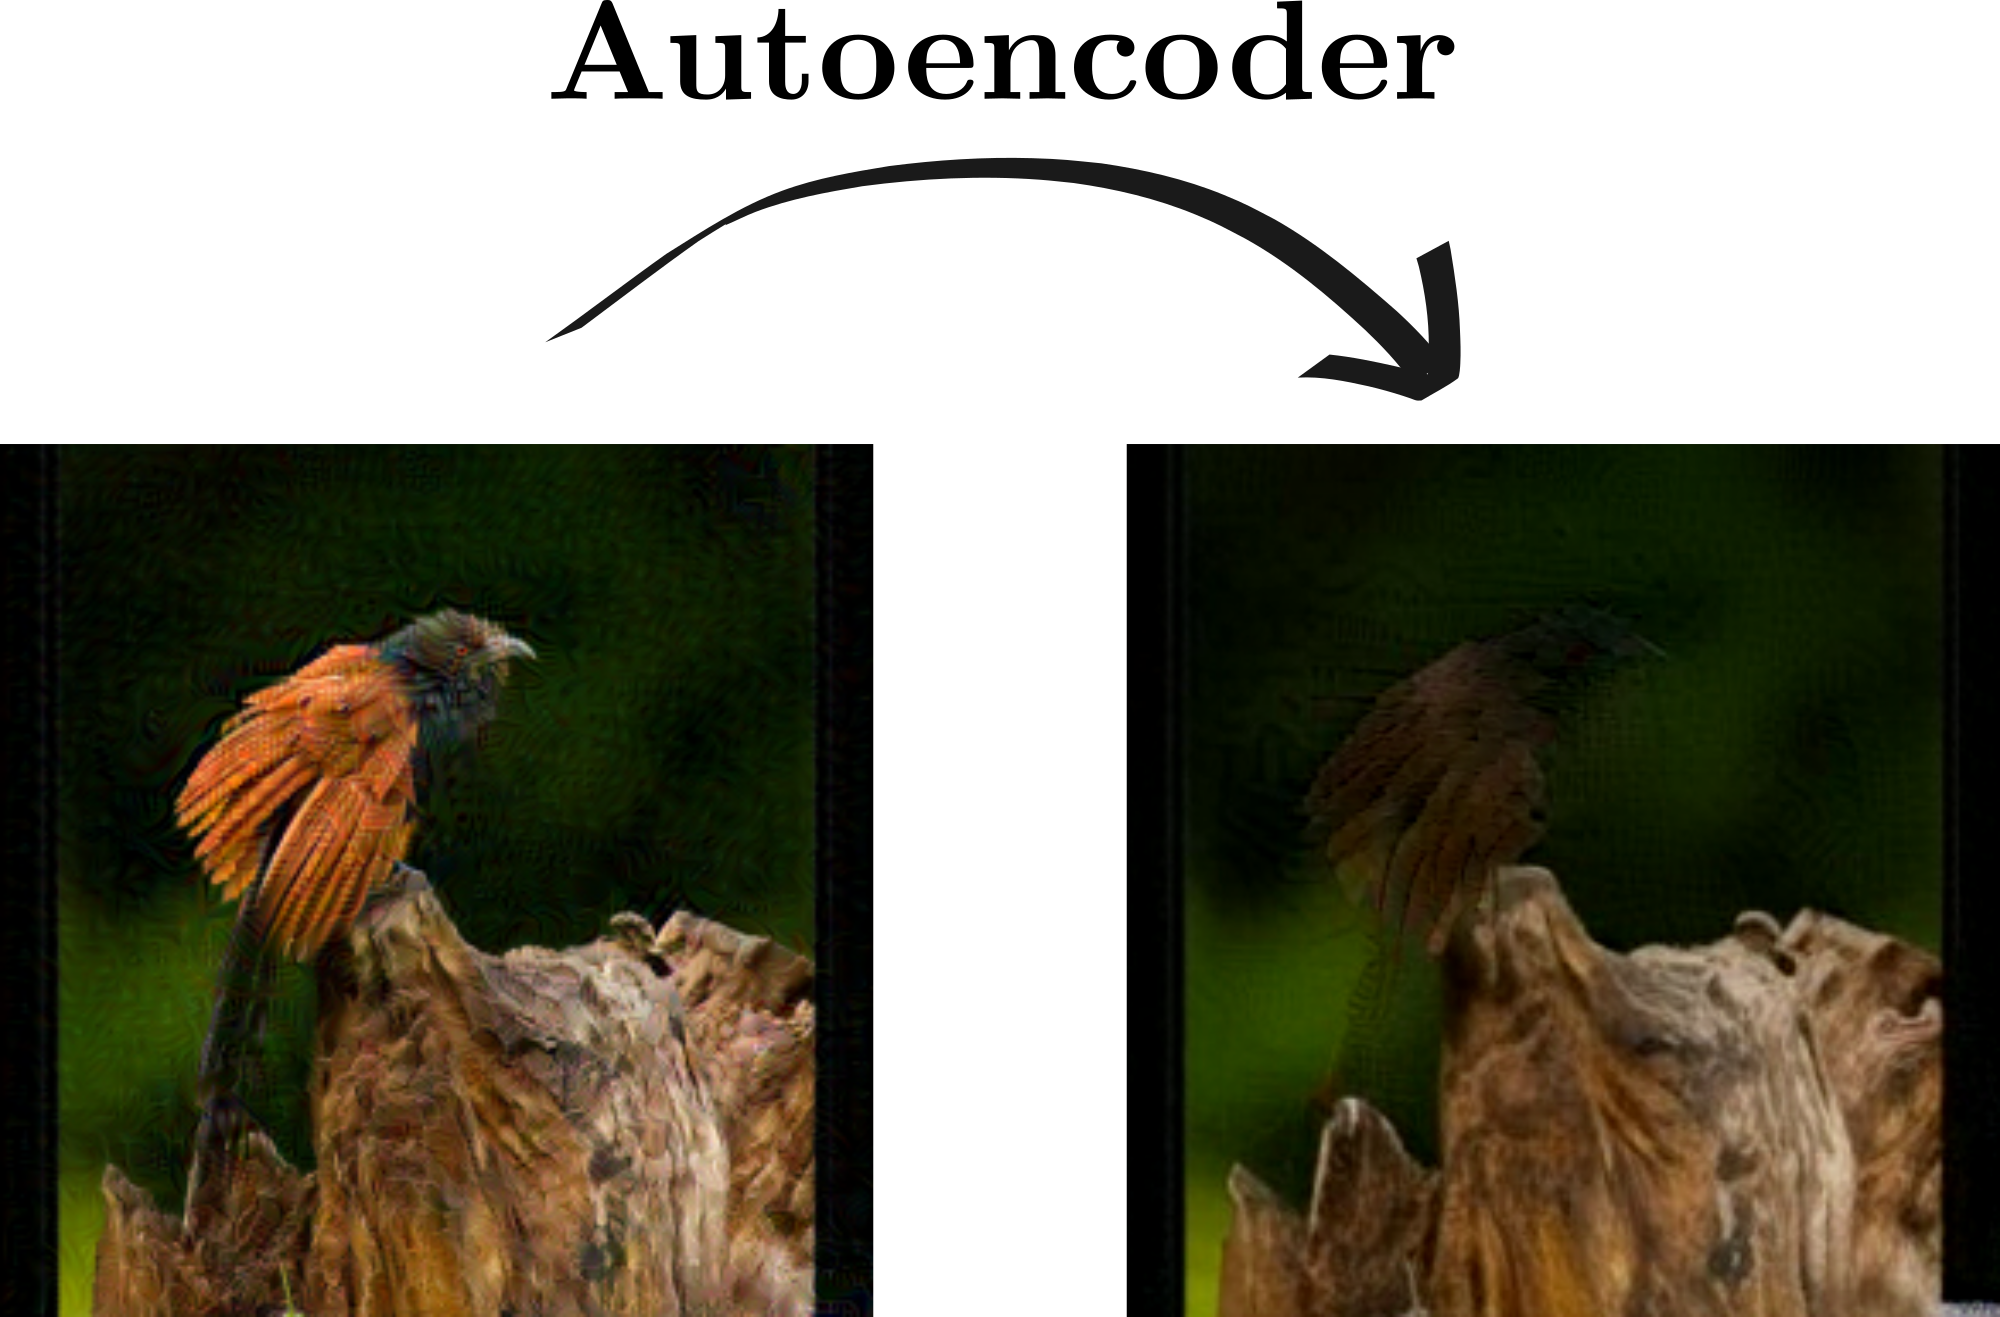
\includegraphics[width=0.8\linewidth]{../images/bird-no-bird.png}
        }
    \end{center}

    \vfill


    \begin{minipage}{0.3\textwidth}
        \textit{Author} \\
        Diego \textsc{Dorn}
    \end{minipage}
    ~
    
\includegraphics[width=3cm]{epfl.png}
    ~
    \begin{minipage}{0.3\textwidth}
        \begin{flushright}
            \textit{Supervisor} \\
            Clément \textsc{Hongler}
        \end{flushright}
    \end{minipage}
    \vspace{1cm}

    \vspace*{-3cm}
\end{center}
\end{titlepage}

% \listoftodos[Remaining to be done]
% \newpage


% \setcounter{section}{-1}
\section*{Introduction}
\addcontentsline{toc}{section}{Introduction}

Machine learning models take more and more importance in our society.
From recommender systems of social media and search engines,
to automated screening of job and loan applications,
from power grid management
to general-purpose generative models,
we seem to be going towards a world where more and more decisions
are automated.

However, if we want the mass deployment of those systems
to not be accompanied by more than normal accidents,
we still need to understand better how those systems work,
and especially how they fail.\footnote{
  This is, however, obviously not sufficient
  and other ingredients such as a good democratic control loop,
  legal frameworks and avoiding concentration of power
  are also necessary.}

In this project, I focused on a specific kind of failure:
adversarial attacks. Adversarial attacks are likely the most
studied failure mode of machine learning algorithms.
They are small perturbations
of the input of a machine learning model that
fools the model into producing a very different output.

The initial goal of the project was to find transferable attacks
on the visual components of multimodal large language models,
however, we switched to attacking image autoencoders.
Autoencoders are a class of neural networks that are trained
to compress and reconstruct their input, and can be used
as a defence mechanism against some adversarial attacks.

The project is divided into three parts. In the first part,
we show different adversarial attacks on classifiers,
before applying them to autoencoders in the second part,
where we show that autoencoders can completely
transform their input into another image.
Finally, in the third part, we present
a novel finding on the norm of activations of
autoencoders when under an attack to transform their input.


% Should I talk about the illusion of safety?

% \cite{szegedy2013intriguing,goodfellow2014explaining,liu2021survey}.
% \todo{Check the papers}

% \begin{multicols}{2}
  \clearpage
  \tableofcontents
% \end{multicols}

\clearpage
\section*{Conventions}
\addcontentsline{toc}{section}{Conventions}

Throughout this document, we adopt a set of conventions and notations.
\begin{itemize}
  \item $\Xx \subset \R^n$ is the set in which datapoints live.
  \item $\Yy$ is a space of labels, which will most of the time be categorical,
    i.e. $\Yy = \set{0, 1}$ or $\Yy = \set{\text{cat}, \text{dog}, \text{boat}}$.
  \item Loss functions are denoted by $\Ll$.
  \item We write $\norm{\cdot}$ for the euclidean norm on $\R^n$,
    and $\norm{\cdot}_p$ for the $p$-norm on $\R^n$.
    As a reminder, for $x \in \R^n$, $\norm{x}_\infty = \max_{i=1}^n \abs{x_i}$.
\end{itemize}


\clearpage

\section{Attacking classifiers}
The common knowledge is that neural networks are vulnerable to adversarial attacks
and adversarial attacks are easy to find \cite{szegedy2013intriguing,goodfellow2014explaining,liu2021survey}.
The first thing I wanted to do was to verify this in practice. Can I easily
attack any classifier outside of the well-defined confines of a classroom
or a paper for which a lot of work was put into?

\subsection{Setup}
I used three different models and datasets throughout this project.
The code of every experiment is available at \url{
  https://github.com/ddorn/autoencoder-attacks
}.

\paragraph{MNIST}
The smallest dataset I used is the MNIST dataset \cite{LeCun1998GradientbasedLA},
with a small convolutional classifier achieving $98.8\,\%$ accuracy implemented in pytorch \cite{tuomaso2022trainmnistfast}.0

\paragraph{CIFAR-10}
The second dataset is the CIFAR-10 dataset \cite{Krizhevsky2009LearningML},
with a convolutional classifier acheiving $92.8 \%$ accuracy \cite{999912022cifar10fastsimple}.

\begin{figure}[h]
  \centering
  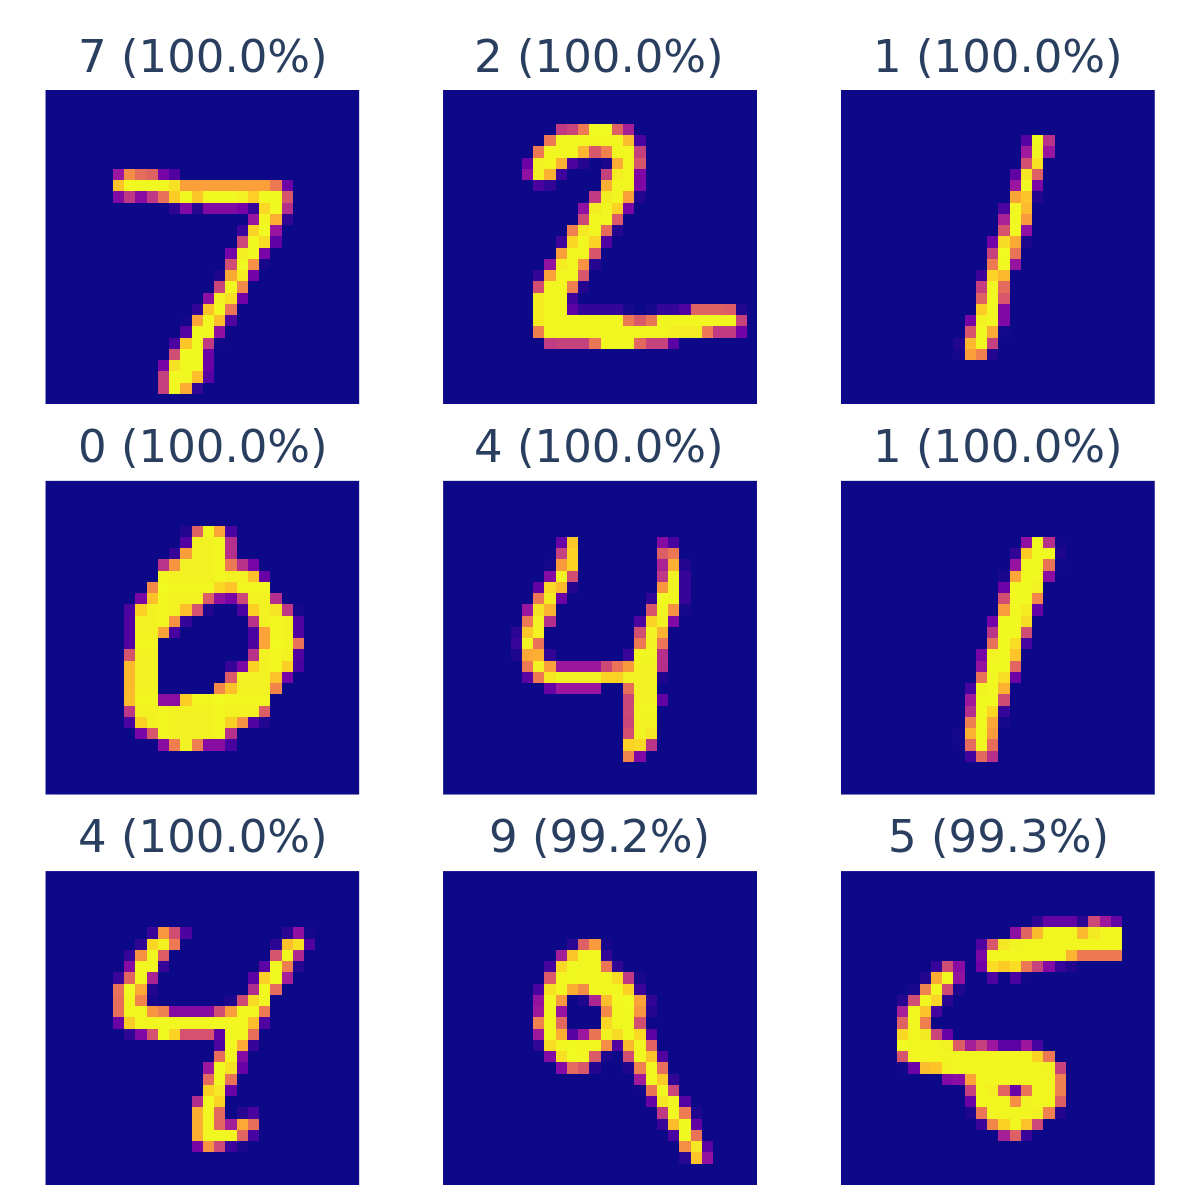
\includegraphics[width=0.45\textwidth]{../images/sample_MNIST.png}
  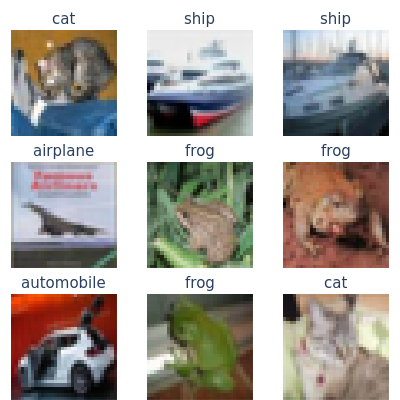
\includegraphics[width=0.45\textwidth]{../images/sample_CIFAR10.png}
  \caption{
    The first 9 test images of
    the MNIST dataset (left)
    the CIFAR-10 dataset (right).
    The confidence of the classifier is shown in parentheses.}
  \label{fig:mnist_cifar10_samples}
\end{figure}


\paragraph{ImageNet}
The third dataset is ImageNet \cite{Deng2009ImageNetAL}, with a ResNet-50 classifier
achieving $77\,\%$ top-1 accuracy \cite{He2015DeepRL}.

\begin{figure}[h]
  \centering
  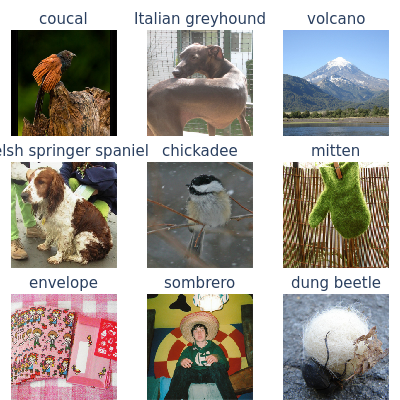
\includegraphics[width=0.45\textwidth]{../images/sample_ImageNet.png}
  \caption{The first 9 test images of the ImageNet dataset.
    The confidence of the classifier is shown in parentheses.}
  \label{fig:imagenet_samples}
\end{figure}


\subsection{Fast gradient sign method}
The simplest attack is the fast gradient sign method (FGSM) \cite{goodfellow2014explaining}.
FGSM works by linearizing the loss function around the input and
computing the exact maximum of the linearized loss function.

This attack requires only one forward and one backward pass through the network
to find a small perturbation of an image that can (potentially) fool the classifier.

What is small? We usually constrain the norm of the perturbation to
a small value $\epsilon$. The norm used can be the $l_\infty$ norm,
for $\epsilon = 10 / 255$ or $\epsilon = 4 / 255$ are common values,
or the $l_0$, $l_1$ or $l_2$ norm.
Clearly, the four norms produce different constraints and should be chosen
depending on the context:
\begin{itemize}
  \item $l_\infty$ is a natural choice and corresponds to changing each
    pixel value by at most $\epsilon$.
    % If $\epsilon \leq 4 / 255$, the perturbation is not visible to the human eye.
  \item Using the $l_0$ norm means to change at most $\epsilon$ pixels. This
    can be one-pixel attacks \cite{Su2017OnePA},
    attacks that change a small number of pixels,
    or patch attacks \cite{Brown2017AdversarialP}.
  \item $l_1$ and $l_2$ constraints can be used when it is fine if
    some pixels are completely changed, but not too many are changed
    a lot.
\end{itemize}

The fast gradient sign method is an untargeted attack, meaning that
the goal is to find a perturbation that changes the prediction of the classifier,
but not to force the classifier to predict a specific label.
It is defined as follows.

\begin{definition}
  Let $f$ be a classifier and $x \in \Xx$ an input with label $y \in \Yy$.
  The \emph{fast gradient sign method} is the attack that computes
  \[
    %\Adversarial{x}
    x_{\text{FGSM}}
      = x + \epsilon \cdot \Sign \Par{\nabla_x \Ll(f(x), y)}
  \]
  where $\Ll$ is the loss function used to train $f$,
  and $\epsilon$ is the desired $l_\infty$ norm of the perturbation.
\end{definition}

We show an example of the attack on the first test image for each of the
datasets, with the top 5 categories shown in
\autoref{fig:fgsm_examples_mnist}, \autoref{fig:fgsm_examples_cifar10}
and \autoref{fig:fgsm_examples_imagenet}.

% A full page for the figure below, without page numbers
\begin{figure}[H]
  \centering
  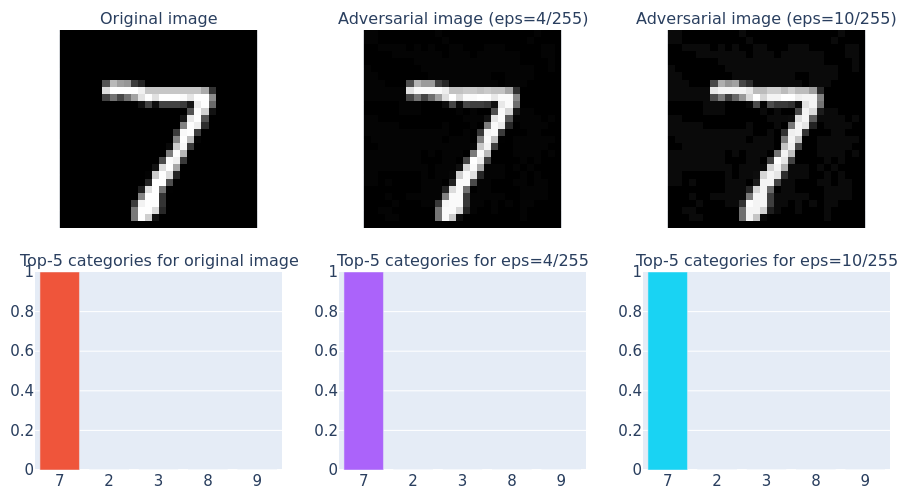
\includegraphics[width=0.9\textwidth]{../images/fgsm_example_MNIST.png}
  \caption{Example of a (non-successful) FGSM attack on MNIST.}
  \label{fig:fgsm_examples_mnist}
\end{figure}

\begin{figure}[H]
  \centering
  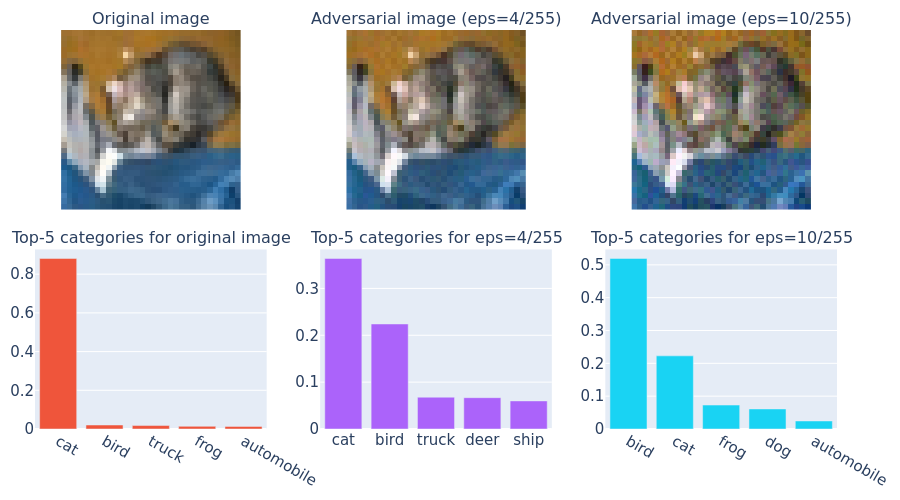
\includegraphics[width=0.9\textwidth]{../images/fgsm_example_CIFAR10.png}
  \caption{Example of an FGSM attack on CIFAR10.}
  \label{fig:fgsm_examples_cifar10}
\end{figure}

\begin{figure}[H]
  \centering
  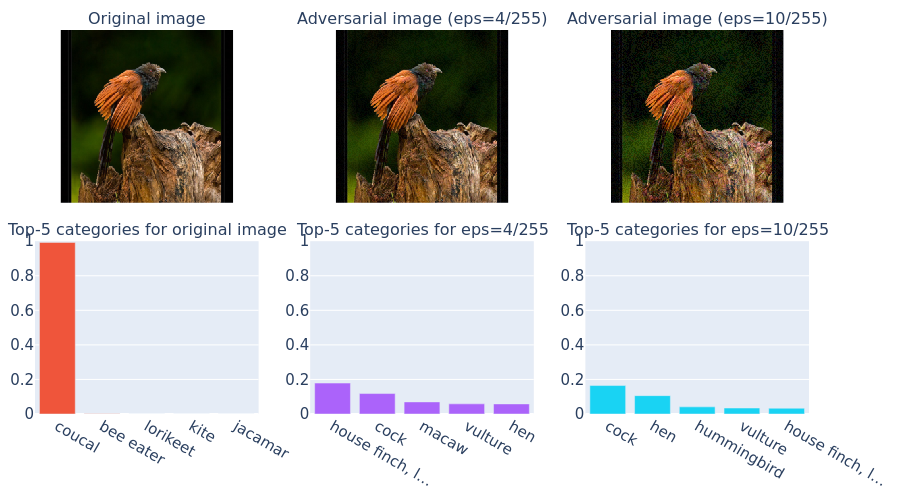
\includegraphics[width=0.9\textwidth]{../images/fgsm_example_ImageNet.png}
  \caption{Example of an FGSM attack on ImageNet.}
  \label{fig:fgsm_examples_imagenet}
\end{figure}

The attack seems to not work for the image from MNIST, but works well
on the one from CIFAR10 and ImageNet.
Is this the case for all images?

So I take the three classifiers, a thousand test images from each dataset,
compute the gradient of the loss with respect to the input image
and add $\e = 10 / 255$ times the sign of the gradient to the image.
This gives a thousand adversarial images for each task and
we can see the accuracy of the clean versus the adversarial images
in \autoref{fig:fgsm_eps10_agregate}.

\begin{figure}[H]
  \centering
  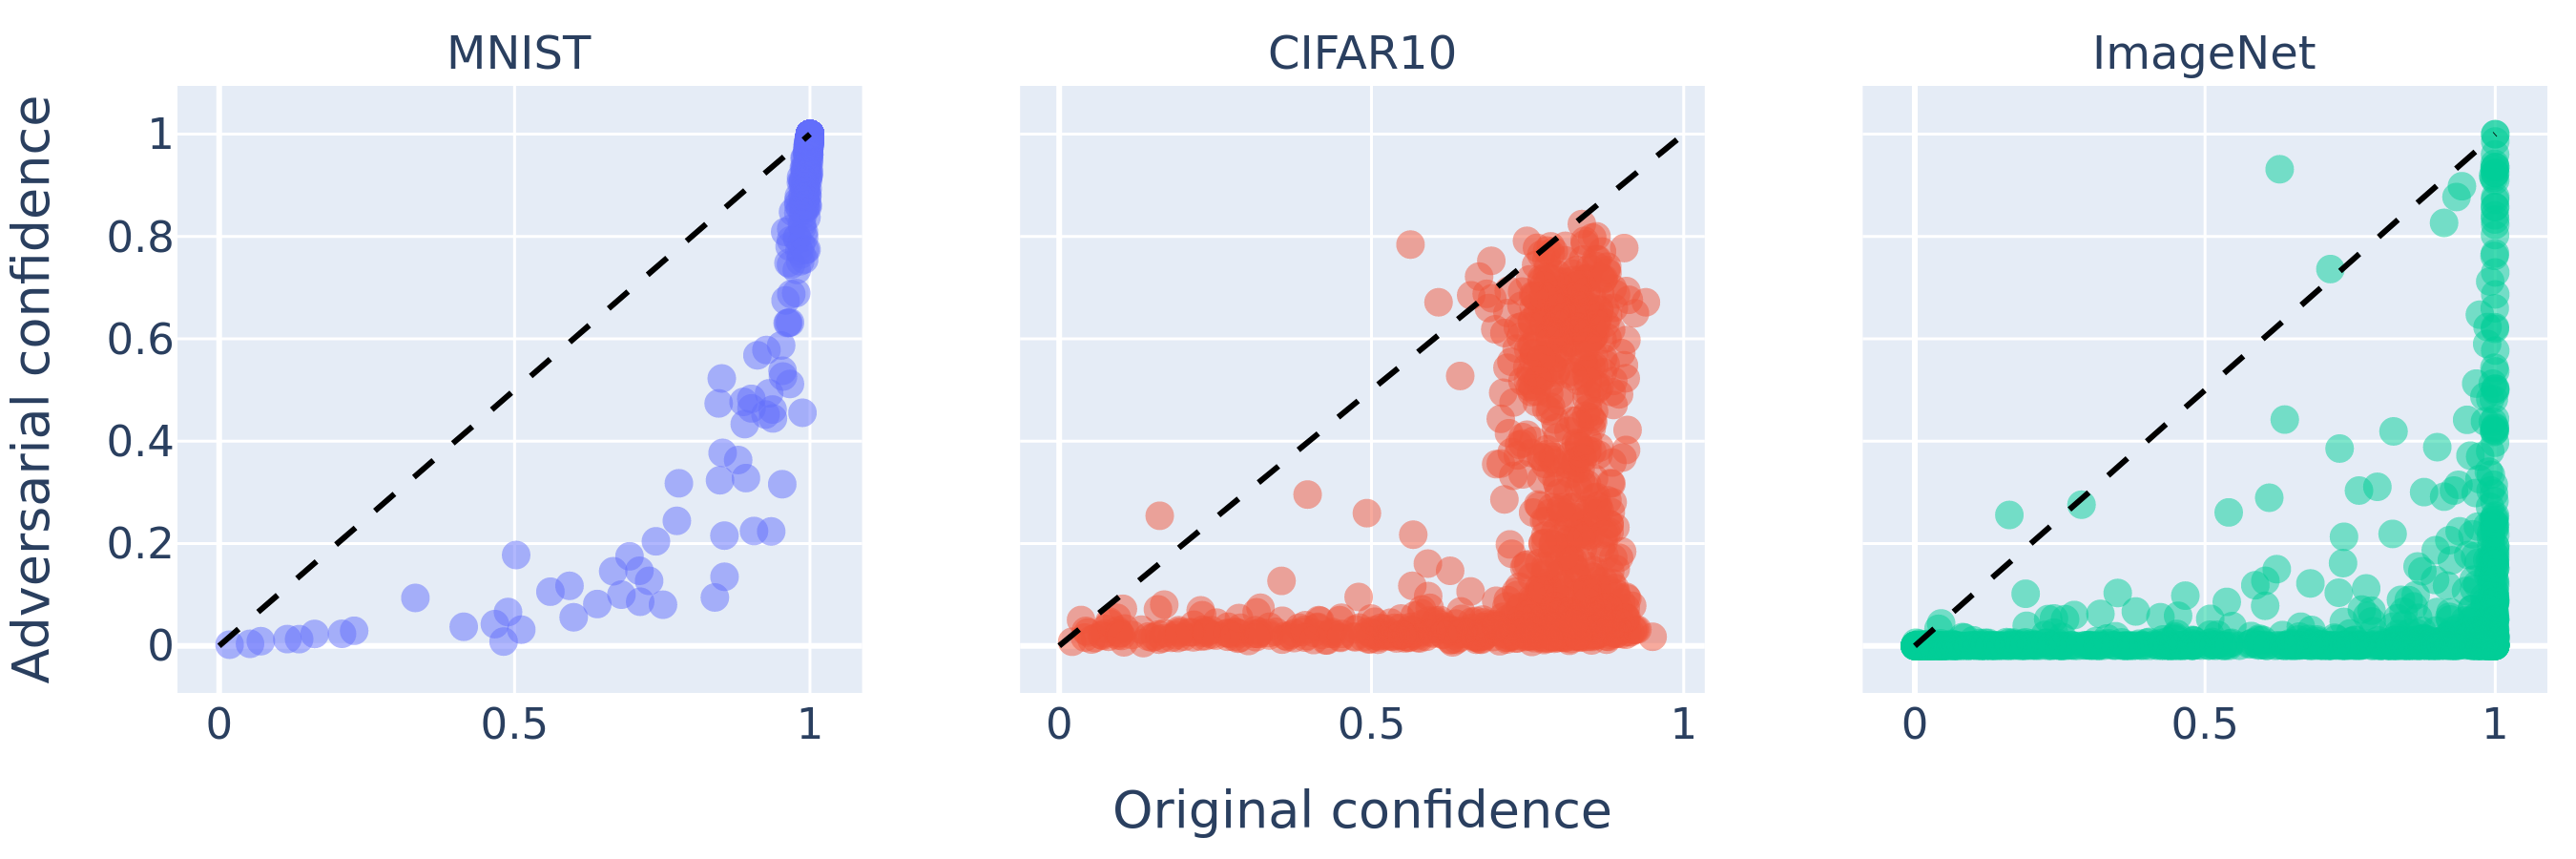
\includegraphics[width=0.9\textwidth]{../images/fgsm_strength.png}
  \caption{Confidence of the three classifiers in the correct label of
    a 1000 test images before and after an FGSM attack with $\epsilon = 10 / 255$.
    The black line corresponds to no change in confidence.
  }
  \label{fig:fgsm_eps10_agregate}
\end{figure}

We can see that, on aggregate, it works very well on ImageNet and CIFAR10,
and less well on MNIST. This can likely be attributed to the fact that
images from CIFAR10 and ImageNet are larger than MNIST and with three
colour channels instead of one. The larger size allows for more ways to
find a path towards the decision boundary.
The sizes can be found in \autoref{table:dataset_sizes}.

\begin{table}[h]
  \centering
  \begin{tabular}{l|cccc}
    & MNIST & CIFAR10 & ImageNet \\ \hline
    Clean accuracy	& 98.9\,\%	& 92.8\,\%	& 77.2\,\%	& \\
    Accuracy $\epsilon=4/255$	& 98.8\,\%	& 87.2\,\%	& 50.2\,\%	& \\
    Accuracy $\epsilon=10/255$	& 98.8\,\%	& 76.8\,\%	& 28.2\,\%	& \\
    Image size & $1 \times 28 \times 28$ & $3 \times 32 \times 32$ & $3 \times 256 \times 256$\footnotemark
  \end{tabular}
  \caption{Top-1 accuracy before and after FGSM attack on a thousand images.}
  \label{table:dataset_sizes}
\end{table}

\footnotetext{
  ImageNet has images of different sizes, but were resized and cropped
  to $256 \times 256$. This is different from the original paper
  \cite{He2015DeepRL} which used $224 \times 224$ images,
  but the classifier still achieves good accuracy.
  This design choice comes from the fact that the autoencoder
  used in the next section cannot take images smaller than $256 \times 256$.
}

\todo{Check that the footnote is on the same page as the figure}

\subsection{Variants of the fast gradient sign method}
The fast gradient sign method is a simple and efficient attack,
but can be made more powerful in multiple ways.

\paragraph{Targeted attacks}
The fast gradient sign method is an untargeted attack,
meaning that the goal is to find a perturbation that changes the prediction of the classifier,
but not to force the classifier to predict a specific label.
However, the attack can be easily modified to be targeted,
as is the case with most attacks.

\begin{definition}
  Let $x \in \Xx$ be any input and $y \in \Yy$ be any label
  (but likely not the label of $x$).
  Then, the \emph{targeted fast gradient sign method} is defined as follows.
  \[
    x_{\text{FGSM}} = x - \epsilon \cdot \Sign \Par{\nabla_x \Ll(f(x), y)}
  \]
  Where $\Ll$ is the loss function used to train $f$,
  and $\epsilon$ is the desired $l_\infty$ norm of the perturbation.
\end{definition}

Notice the minus sign instead of the plus sign in the untargeted attack:
we want the loss, evaluated with the target (wrong) label
to decrease. Before, we wanted the loss, evaluated with the correct label
to increase.

\paragraph{Iterative fast gradient sign method}
Instead of adding \e times the sign of the gradient, we can iterate
$N$ times and add $\e / N$ times the sign of the gradient at each step.
This is called the iterative fast gradient sign method.
In our experiments, this managed to find adversarial images with
smaller perturbations, and for harder attack targets it
is necessary to iterate on the attack multiple times.

% \paragraph{Iterative gradient ascent}
% Instead of taking the sign of the gradient,
% we can take the gradient itself, multiply it by a learning rate,
% and add it to the image.


\paragraph{Transferable attacks}
The fast gradient sign method is a white box attack,
meaning that it requires access to the weights of the model
to perform the attack. In practice, a lot of models are proprietary,
or at least not easily accessible, but this does not mean that
they are safe from adversarial attacks.

Indeed, it is possible to create attacks that are transferable
to other models, meaning that the adversarial images produced
by the attack on one model are also adversarial images for another model.
This can be used for instance to attack a large model, with
only access to a smaller model.
Attacks on vision models tend to be transferable by default,
and can even transfer, in a weak sense, to humans \cite{Elsayed2018AdversarialET}.

However, stronger transferable attacks can be found by
attacking multiple models at once, that is, by using
the mean of the loss of multiple models instead of the loss of one model.
While this was the topic I initially started to work on,
it will not be the focus of the rest of this report.


% Competition \cite{Kurakin2018AdversarialAA}









\clearpage

\section{Attacking autoencoders}

Autoencoders have been suggested as a defence mechanism against adversarial attacks.
\todo{add citation}

\subsection{Autoencoders}

Autoencoders were introduced by \cite{hinton2006reducing} as a way to learn
a low-dimensional representation of data.
They are a class of neural networks that are trained to reconstruct their input,
and are composed of two deep neural networks, an encoder and a decoder with a bottleneck in between
as shown in \autoref{fig:autoencoder}.

\begin{figure}[h]
  \centering
  \begin{tikzpicture}
    % Encoder, a trapeze
    \draw[atomictangerine, fill=atomictangerine!20]
      (0, 0) -- (0, 4) -- (4, 3) -- (4, 1) -- cycle;
    \node[] at (2, 2) {Encoder};
    % Bottleneck, vertical text, no shape
    \node[rotate=-90] at (4.5, 2) {Bottleneck};
    % Decoder, a trapeze
    \draw[airforceblue, fill=airforceblue!20]
      (5, 1) -- (5, 3) -- (9, 4) -- (9, 0) -- cycle;
    \node[] at (7, 2) {Decoder};

    % Text input on the left, vertical
    \node[rotate=-90] at (-1, 2) {Input}
      edge[->, thick] (-0, 2);
    % Text output on the right, vertical
    \node[rotate=-90] at (10, 2) {Output}
      edge[<-, thick] (9, 2);
  \end{tikzpicture}
  \caption{Overview of the autoencoder architecture}
  \label{fig:autoencoder}
\end{figure}

The \emph{encoder} takes a high dimensional data point as input,
processes it through a series of layers, usually fully connected layers
or a residual network \cite{He2015DeepRL} in the case of visual data,
and outputs a low-dimensional representation of the input.

The \emph{decoder} takes the low dimensional output of the encoder and
processes it similarly through a series of layers,
and outputs a high-dimensional reconstruction of the input.

The \emph{bottleneck} is not a layer, but rather the middle of the autoencoder,
where the activations are the lowest number of dimensions.

\paragraph{Training}
Autoencoders are trained to reconstruct their input,
that is, they learn the identity function. The loss is a natural metric
on the data space, such as the mean squared error for real-valued data.

\begin{definition}
  The \emph{reconstruction loss} for an autoencoder $f$ on an input $x \in \Xx$
  is
  \[
    \Ll_{\text{recon.}}(x) = \norm{x - f(x)}^2
  \]
\end{definition}

To prevent overfitting and to perform a directly useful task,
an autoencoder can be trained to reconstruct a noisy or corrupted
version of the input.
\begin{definition}
  The \emph{denoising loss} for an autoencoder $f$ on an input $x \in \Xx$ is
  \[
    \Ll_{\text{denoising}}(x) = \norm{x - f(x + \e)}^2
  \]
  where \e is a random vector of the same dimension as $x$, of white noise
  whose variance is a hyperparameter of the training setup.

  Note that the denoising loss is stochastic, as it depends on the random
  vector \e. In practice, we use the compute the loss on one sample of \e
  per input.
\end{definition}

\paragraph{Variational AutoEncoders (VAE)}
A specific kind of autoencoder, and the one that will be
used in all of the following experiments,
are variational autoencoders,
introduced by \cite{Kingma2013AutoEncodingVB}
Technically, they are not very different from regular autoencoders,
but they come from a different background than data compression.
Indeed, the hope is that VAEs model the process from which the data was generated.
Often, we expect a datapoint (for instance the image of a leaf) to be determined
only by \textit{a few} variables (for instance, the species of the tree, its age,
the season, the angle at which the picture was taken etc.).
We will call $P$, the vector of those few variables that generate the datapoint.

The encoder of a VAE tries to find some representation of $P$ and outputs two vectors,
$\mu$ and $\sigma$ instead of one, which are interpreted as the mean and the variance
of the prior on $P$, which is assumed to be a normal distribution.

The variable $P \sim \Nn(\mu, \sigma)$ are then sampled
and fed to the decoder that tried to reconstruct what should be
generated from the underlying variables. The decoder thus tries
to model the process that generated the dataset and outputs
a distribution $Q$ over the data space.

\begin{definition}
  Let $f$ be a VAE and $x \in \Xx$ a datapoint.
  It loss on $x$ is composed of two terms,
  the \emph{likelyhood loss} and the \emph{regularisation loss}.
  \[
    \Ll_{\text{vae}}(x) =
      \underbrace{\IP(x \mid f(x))}
        _{\text{likelyhood loss}}
      + \underbrace{\KLdiv{P}{\Nn(0, 1)}}
        _{\text{regularisation loss}}
  \]

\end{definition}

\begin{remark}
  The KL divergence is a measure of how different two distributions are.
  In this case, it is used to measure how far the prior on $P$ is from
  the standard normal distribution.
  \[
    \KLdiv{P}{Q} = \int_{\Xx} P(x) \log \frac{P(x)}{Q(x)} \,\dd x
  \]

  Here we can use the fact that both $P$ and $Q$ are $n$-dimensional normal distributions
  to compute the KL divergence in closed form.
  \[
    \KLdiv{\Nn(\mu, \sigma)}{\Nn(0, 1)}
    = \frac{-1}{2n} \sum_{i=1}^{n} \Par{
      1 + \log \sigma_i^2 - \mu_i^2 - \sigma_i^2
    }
  \]
\end{remark}

Here, the likelihood loss is conceptually equivalent to
the reconstruction loss of a regular autoencoder,
and the regularisation loss is used to
have a latent representation that is close to a normal distribution.
It makes it easier to sample latent representations and
corresponds to the assumption that the underlying variables
are normally distributed.

\subsection{Setup}
I used two different variational autoencoders, one for each dataset and classifier.


\paragraph{MNIST}
On the MNIST dataset, I trained a small convolutional autoencoder with a bottleneck of size 4,
which reconstructs the images with an average per-pixel error of $7.3\,\%$.
\todo{Show architecture}

% \paragraph{CIFAR-10}
% On the CIFAR-10 dataset, I trained a medium convolutional autoencoder with a bottleneck of size ???,
% which reconstructs the images with an average per-pixel error of $???$.
% \todo{add error rate}

\paragraph{ImageNet}
On the ImageNet dataset, I used \texttt{stabilityai/sd-vae-ft-mse}, a pretrained autoencoder from StabilityAI
\cite{stabilityai_sdvaeftmse} with $83.8\text{M}$ parameters.
It has a bottleneck of size 2048 and reconstructs the images with an average per-pixel error of $3.3\,\%$.


\paragraph{}Note: In the following, every use the term \textit{autoencoder}
refers to a variational autoencoder.




\subsection{Autoencoders as a defence mechanism}
Autoencoders can be used to prevent adversarial attacks
against classifiers by prepocessing images through the autoencoder.
The setup is shown in \autoref{fig:ae_defense}.

\begin{figure}[h]
  \centering

  \begin{tikzpicture}[scale=0.8]
    \begin{scope}[local bounding box=autoencoder]
      % Encoder
      \draw[atomictangerine, fill=atomictangerine!20]
        (0, 0) -- (0, 4) -- (4, 3) -- (4, 1) -- cycle;
      \node[] at (2, 2) {Encoder};
      % Decoder
      \draw[airforceblue, fill=airforceblue!20]
        (5, 1) -- (5, 3) -- (9, 4) -- (9, 0) -- cycle;
      \node[] at (7, 2) {Decoder};
      \path[->, thick] (4, 2) --
       node[rotate=-90] {Bottleneck}
       (5, 2);
      % \node[rotate=-90, red] (bottleneck) at (4.5, 2) {Bottleneck};
    \end{scope}

    % Box around the autoencoder, spacing of 0.5 around
    \draw[thick, rounded corners=0cm]
      ($(autoencoder.north west) + (-0.5, 0.5)$) rectangle
      ($(autoencoder.south east) + (0.5, -0.5)$);
    % Label for the autoencoder
    \node[anchor=south] at ($(autoencoder.north) + (0, 0.5)$) {Autoencoder};

    % Text input on the left, vertical
    \node[rotate=-90] at (-1, 2) {Input}
      edge[->, thick] (autoencoder.west);

    % Classifier
    \begin{scope}[local bounding box=classifier]
      \draw[awesome!80, fill=awesome!20] (autoencoder.south east)
        ++(1, 0) -- ++(0, 4) -- ++(4, -1) -- ++(0, -2) -- cycle;
      \node[] at (12, 2) {Classifier};
    \end{scope}

    % Arrow from the autoencoder to the classifier
    \draw[->, thick] (autoencoder.east) -- ++(1, 0);

    % Text output on the right, vertical
    \node[rotate=-90] at ($(classifier.east) + (1, 0)$) {Classification}
      edge[<-, thick] (classifier.east);

  \end{tikzpicture}

  \caption{Autoencoder used as a defence against adversarial attacks}
  \label{fig:ae_defense}
\end{figure}

The hope is that an adversarial perturbation of the input
will not pass through the bottleneck of the autoencoder,
and thus will not be able to fool the classifier.
Indeed, the bottleneck is small, and therefore information
constrained, so we expect the autoencoder to
not faithfully reconstruct patterns that it has never seen
during training. In particular, we expect the latent representation
of an adversarial input to be the same as the representation of
the original input, and thus the autoencoder should reconstruct the
original input when fed the adversarial one.

\todo{Maybe add a plot for the distance between latent representations of clean vs adversarial}
% Vary:
% - autoencoder/task
% - pairs of inputs
% Histogram with:
% - line 1: distance between the latent representation of original and adversarial
% - line 2: distance between random pairs
% - line 3: distance between random pairs of the same class



\paragraph{}
Passing the adversarial images from \autoref{table:dataset_sizes},
through the autoencoder, we can see that the autoencoder
lessens the visual noise on the images as seen in \autoref{fig:ae_examples}.
This happens both because the images are compressed then decompressed,
and because the autoencoders were trained to reconstruct noisy images.

\begin{figure}[h]
  \centering
  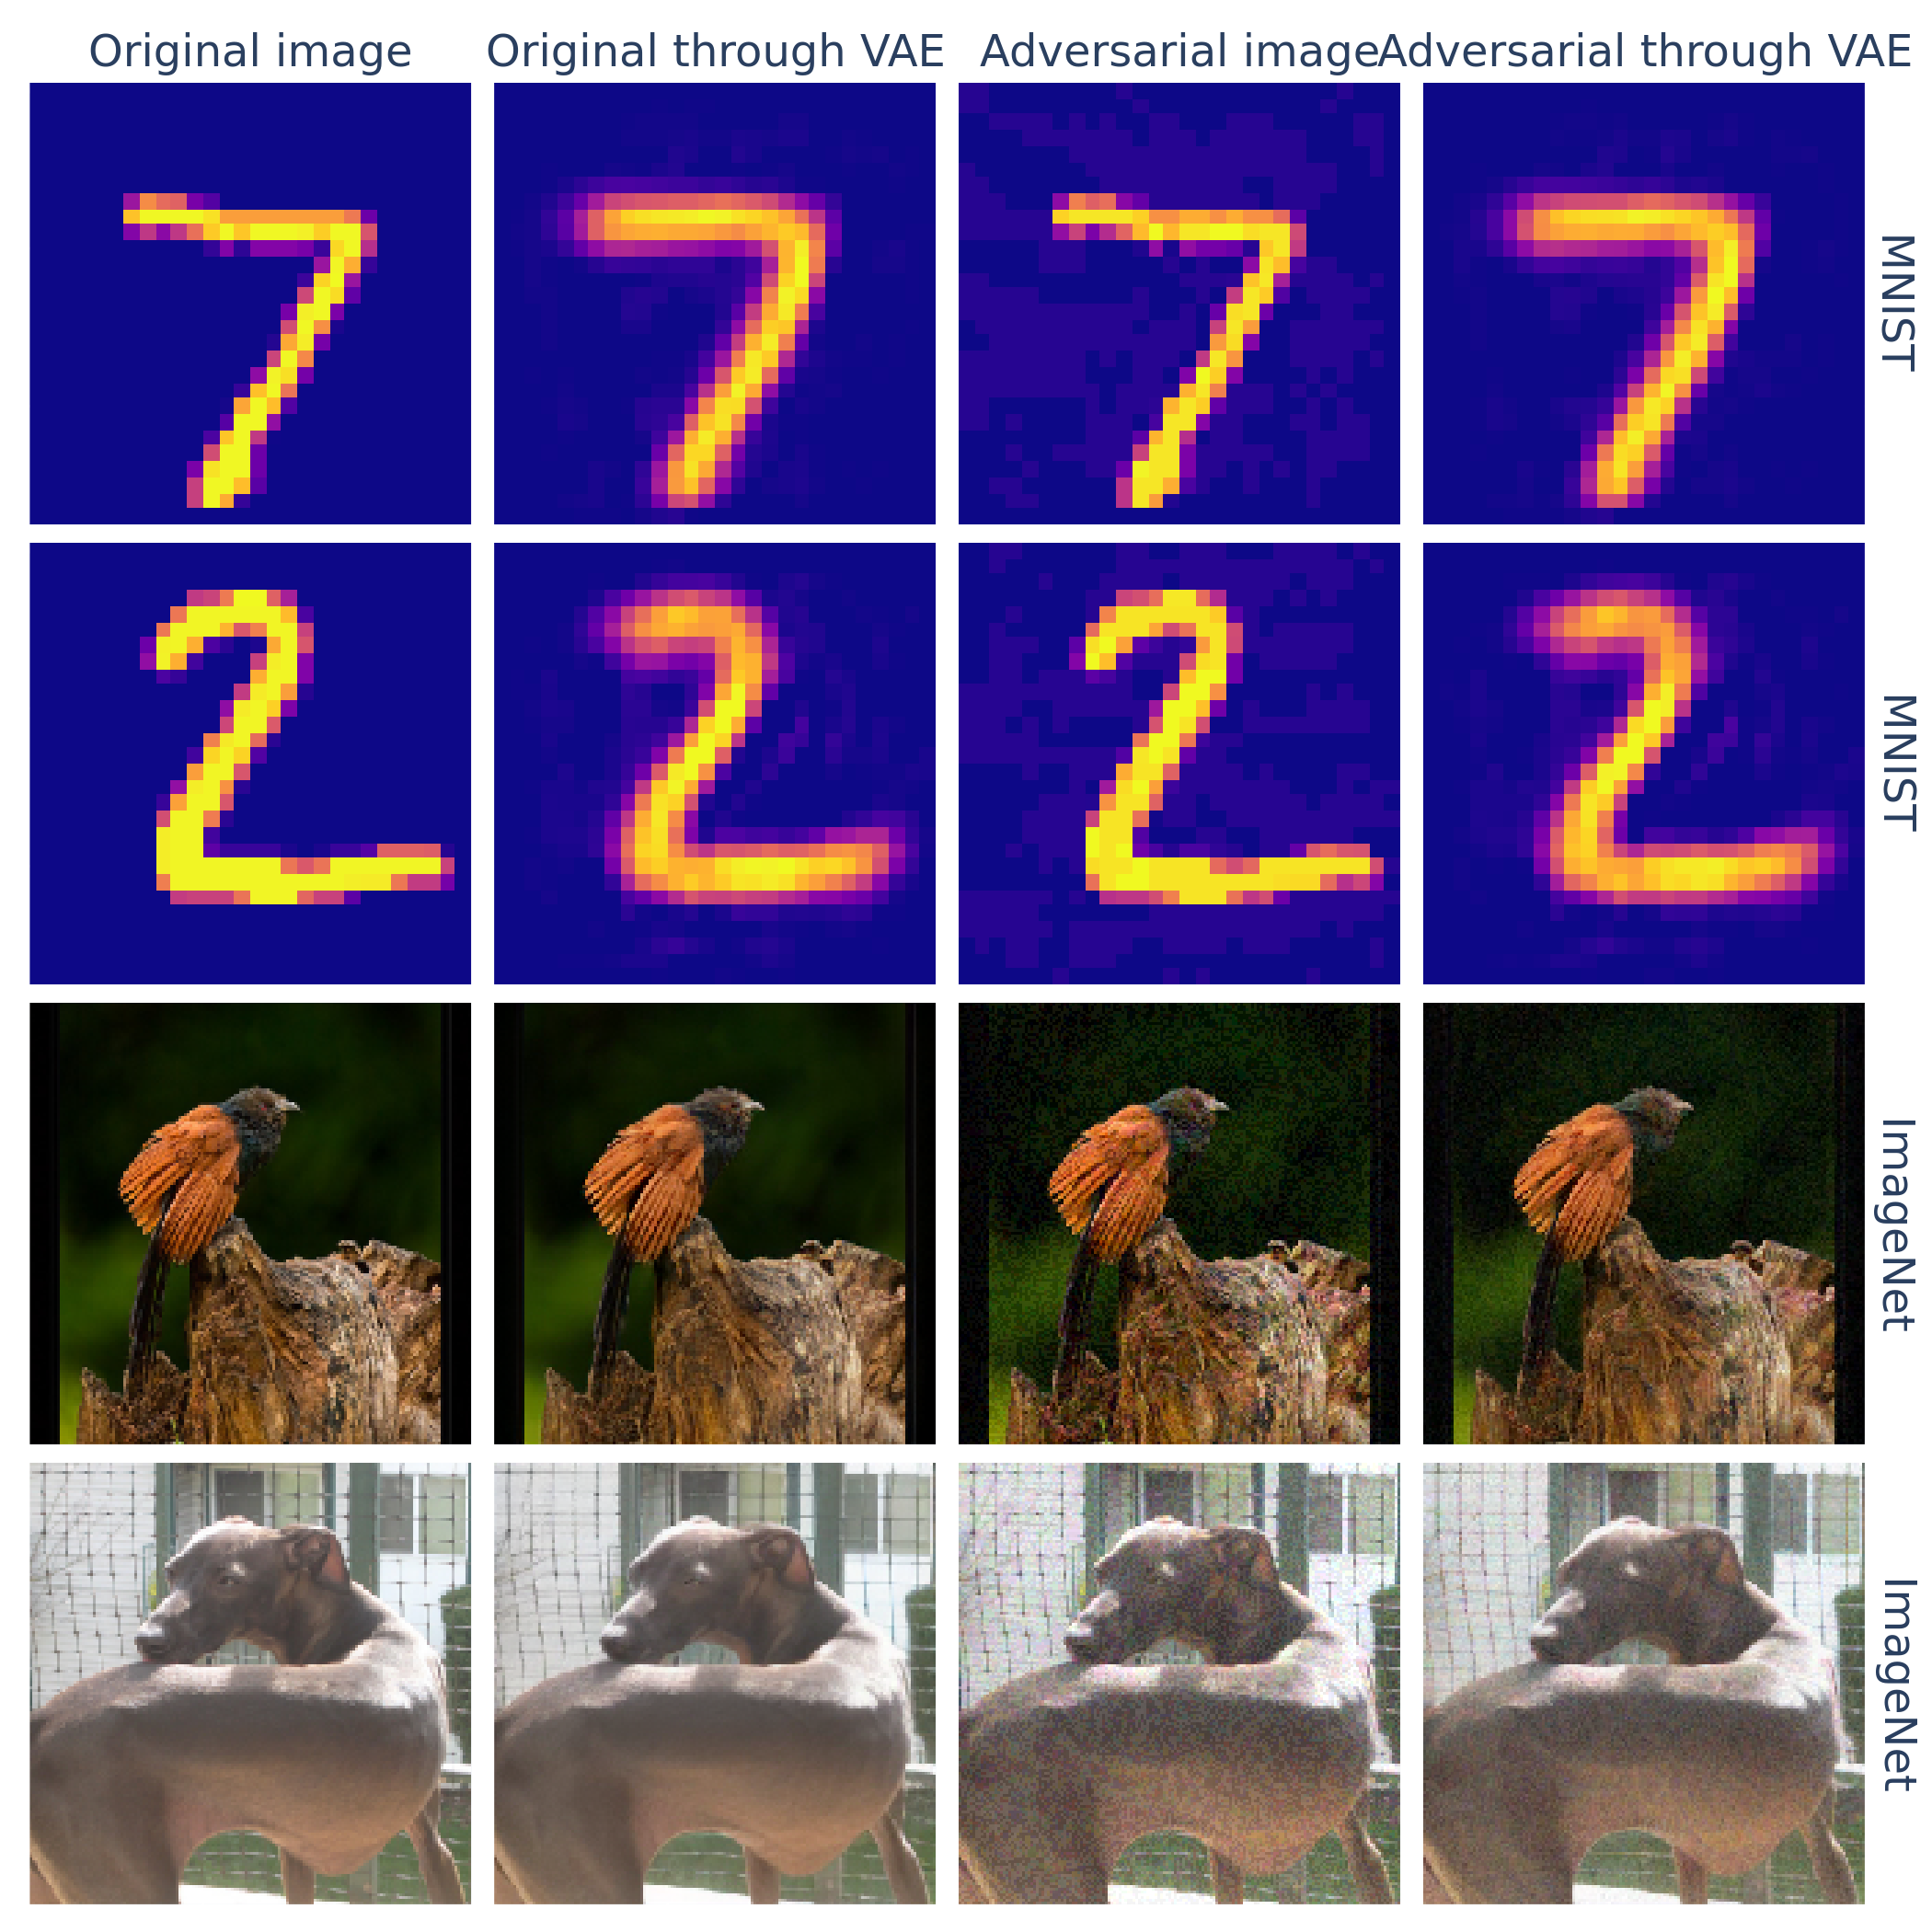
\includegraphics[width=0.9\textwidth]{../images/ae_examples.png}
  \caption{
    Examples of the autoencoder defence.
    \emph{Left}: first 2 images of each dataset.
    \emph{2nd column}: original images passed through the autoencoder.
    \emph{3rd column}: adversarial images, produced by FSGM with $\epsilon = 10/ 255$.
    \emph{Right}: adversarial images passed through the autoencoder.
  }
  \label{fig:ae_examples}
\end{figure}

Passing the image through the VAE also recovers most of the accuracy
of the classifiers, as seen in \autoref{table:ae_examples_confidence}.
However, the base accuracy, on clean images is reduced by a few percent
(about 10\,\% for MNIST and 3\,\% for ImageNet).
This is an instance of the tradeoff between accuracy and robustness.

\begin{table}[h]
  \centering

    \begin{tabular}{c|r|cc}
    & & \multicolumn{2}{c}{Autoencoder} \\
    & & Without & In front \\
    \hline
    \multirow{3}{*}{MNIST}
    &  Clean accuracy			& 98.9\,\%	& 89.1\,\%	\\
    &  Accuracy $\epsilon=4/255$	& 98.8\,\%	& 88.9\,\%	\\
    &  Accuracy $\epsilon=10/255$	& 98.8\,\%	& 89.0\,\%	\\
    \hline
    \multirow{3}{*}{ImageNet}
    &  Clean accuracy			& 77.2\,\%	& 74.7\,\%	\\
    &  Accuracy $\epsilon=4/255$	& 50.2\,\%	& 72.7\,\%	\\
    &  Accuracy $\epsilon=10/255$	& 28.2\,\%	& 69.7\,\%	\\
  \end{tabular}

  \caption{Accuracy of the classifier on the original and autoencoded images.}
  \label{table:ae_examples_confidence}
\end{table}

However, this is a very simple baseline defence, which relies on the attacker
not knowing about the autoencoder, or not having access to it,
and some attacks work even in this case.
\todo{Add reference to the paper that does this}

More sophisticated defences can be designed, and many have been proposed.
One can randomly pick an autoencoder from a pool of autoencoders,
add noise to the input, take the median of the output of many autoencoders,
or use other compression metrics such as JPEG \cite{Shin2017JPEGresistantAI}
or reducing the precision of the image.
\todo{Add reference to the paper that does this}

In any case, even if security through obscurity might work,
it goes against Kerckhoffs's principle \cite{kerckhoffs1883cryptographie},
which states that a system should be secure even if the attacker
knows everything about it, except the secret key.
There is not a nice concept of a secret key here,
but considering the autoencoder as a secret key is not a good idea,
as an autoencoder is too big, with too much information about the world
to be considered secret.





\subsection{Attacking through autoencoders}

In a setting where an attacker knows the autoencoder placed as a defence
in front of the classifier, one can wonder what type of attack exists.
It seemed to me that it would be hard to generate an adversarial perturbation
as the output of an autoencoder since this model has never been trained
to produce this kind of structure. On the other hand, I thought that it would
be easier to make the autoencoder produce an entirely different image.
My advisor expected it to be hard to make an autoencoder produce a different
image, I set out to prove it wrong.

\paragraph{}
There are two natural attacks to try:
\begin{enumerate}
  \item Attacking the composition of the autoencoder and classifier, to
    produce a different label, hoping that it ``fools'' the classifier
    by feeding it an image of something else than the original input.
    In this case, the loss function is the loss of the classifier.
    For an image $x$ and a target label $y$, we have
    \[
      \Ll_1(x, y) = \Ll_{\text{cross.}}(\mathrm{Classifier}(\mathrm{Autoencoder}(x)), y)
    \]
    The attack can also be untargeted, in which case the target label $y$
    is chosen to be the label of the original image $x$ and we search
    for the maximum of the cross entropy loss instead of the minimum.
  \item Attacking the autoencoder directly to produce a different image.
    In this case, the loss function is the reconstruction loss of the autoencoder,
    hover
    For two images $x$ and $x'$, we have
    \[
      \Ll_2(x, x') = \Ll_{\text{rec.}}(\mathrm{Autoencoder}(x), x')
    \]
\end{enumerate}



\begin{figure}[h]
  \centering
  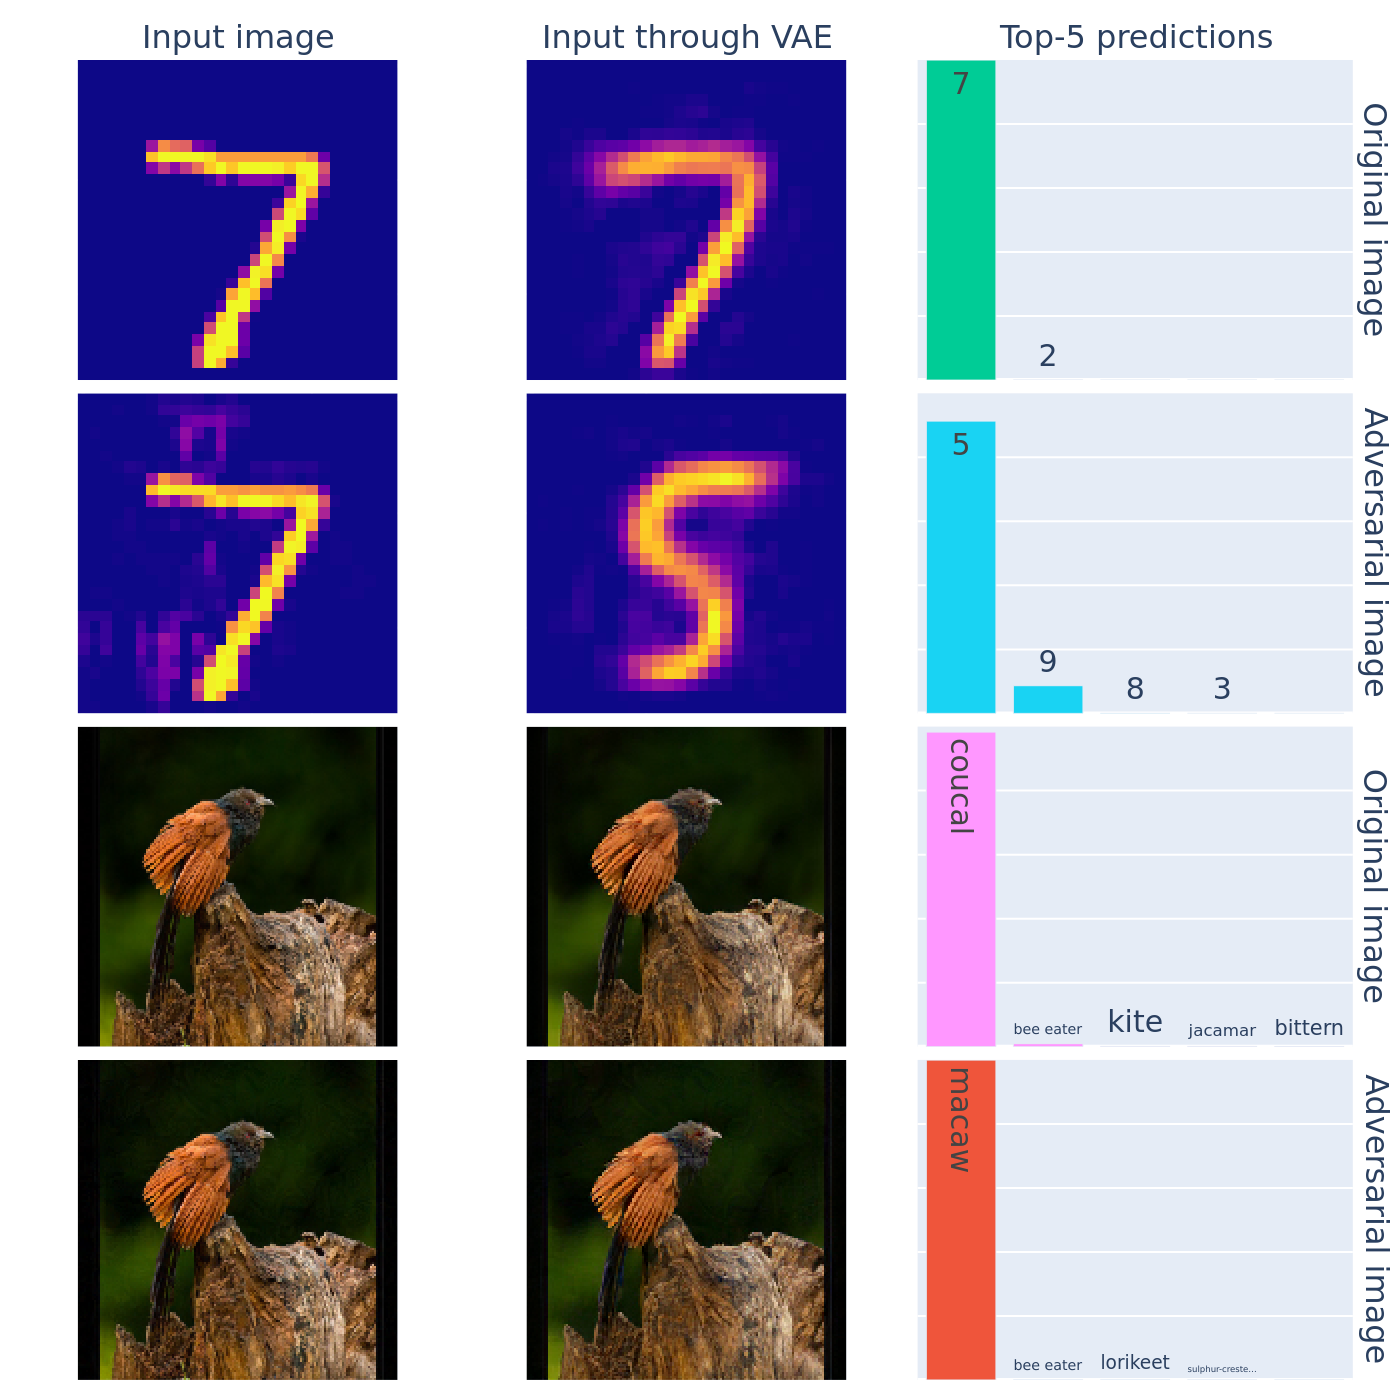
\includegraphics[width=0.9\textwidth]{../images/ae_attack_examples.png}
  \caption{
    Examples of attacks through the autoencoder.
  }
  \label{fig:ae_attack_examples}
\end{figure}


We show in \autoref{fig:ae_attack_examples} two examples of attacks
against the composition of the autoencoder and classifier.
The most interesting thing to note is that the visuals of the
adversarial images are very different on the two datasets:
\begin{itemize}
  \item For MNIST, the autoencoder produces an image that looks like
    a 5 or a 9, which is very different from the initial image of a 7.
  \item For ImageNet, the autoencoder produces an image that is undistinguishable
    from the original image, but the classifier predicts a different label.
\end{itemize}

Therefore, both kinds of attack mechanisms are possible. It is possible to transform an image through an autoencoder
into something that a human would recognise as different
(or at least for this specific small VAE on MNIST), but it is also possible
to make an autoencoder produce an adversarial image.

The attacks being different for the two datasets suggests that
transforming an image is easier on small networks or images
but on larger networks/images it is easier to make the autoencoder
produce and adversarial perturbation.
Before verifying this hypothesis,
\todo{verify this hypothesis}
we need to check if this pattern holds for other autoencoders.

Taking 20 random images from the test set of each dataset,
we can see in \autoref{fig:ae_attack_examples_many} that the pattern
does hold.
% However, note that we filtered out the images for which
% the attack did not succeed in fooling the classifier, which is about
% $??? \%$ of the images for MNIST and $??? \%$ for ImageNet.
% \todo{Compute attack success rate}

\begin{figure}[h]
  \centering
  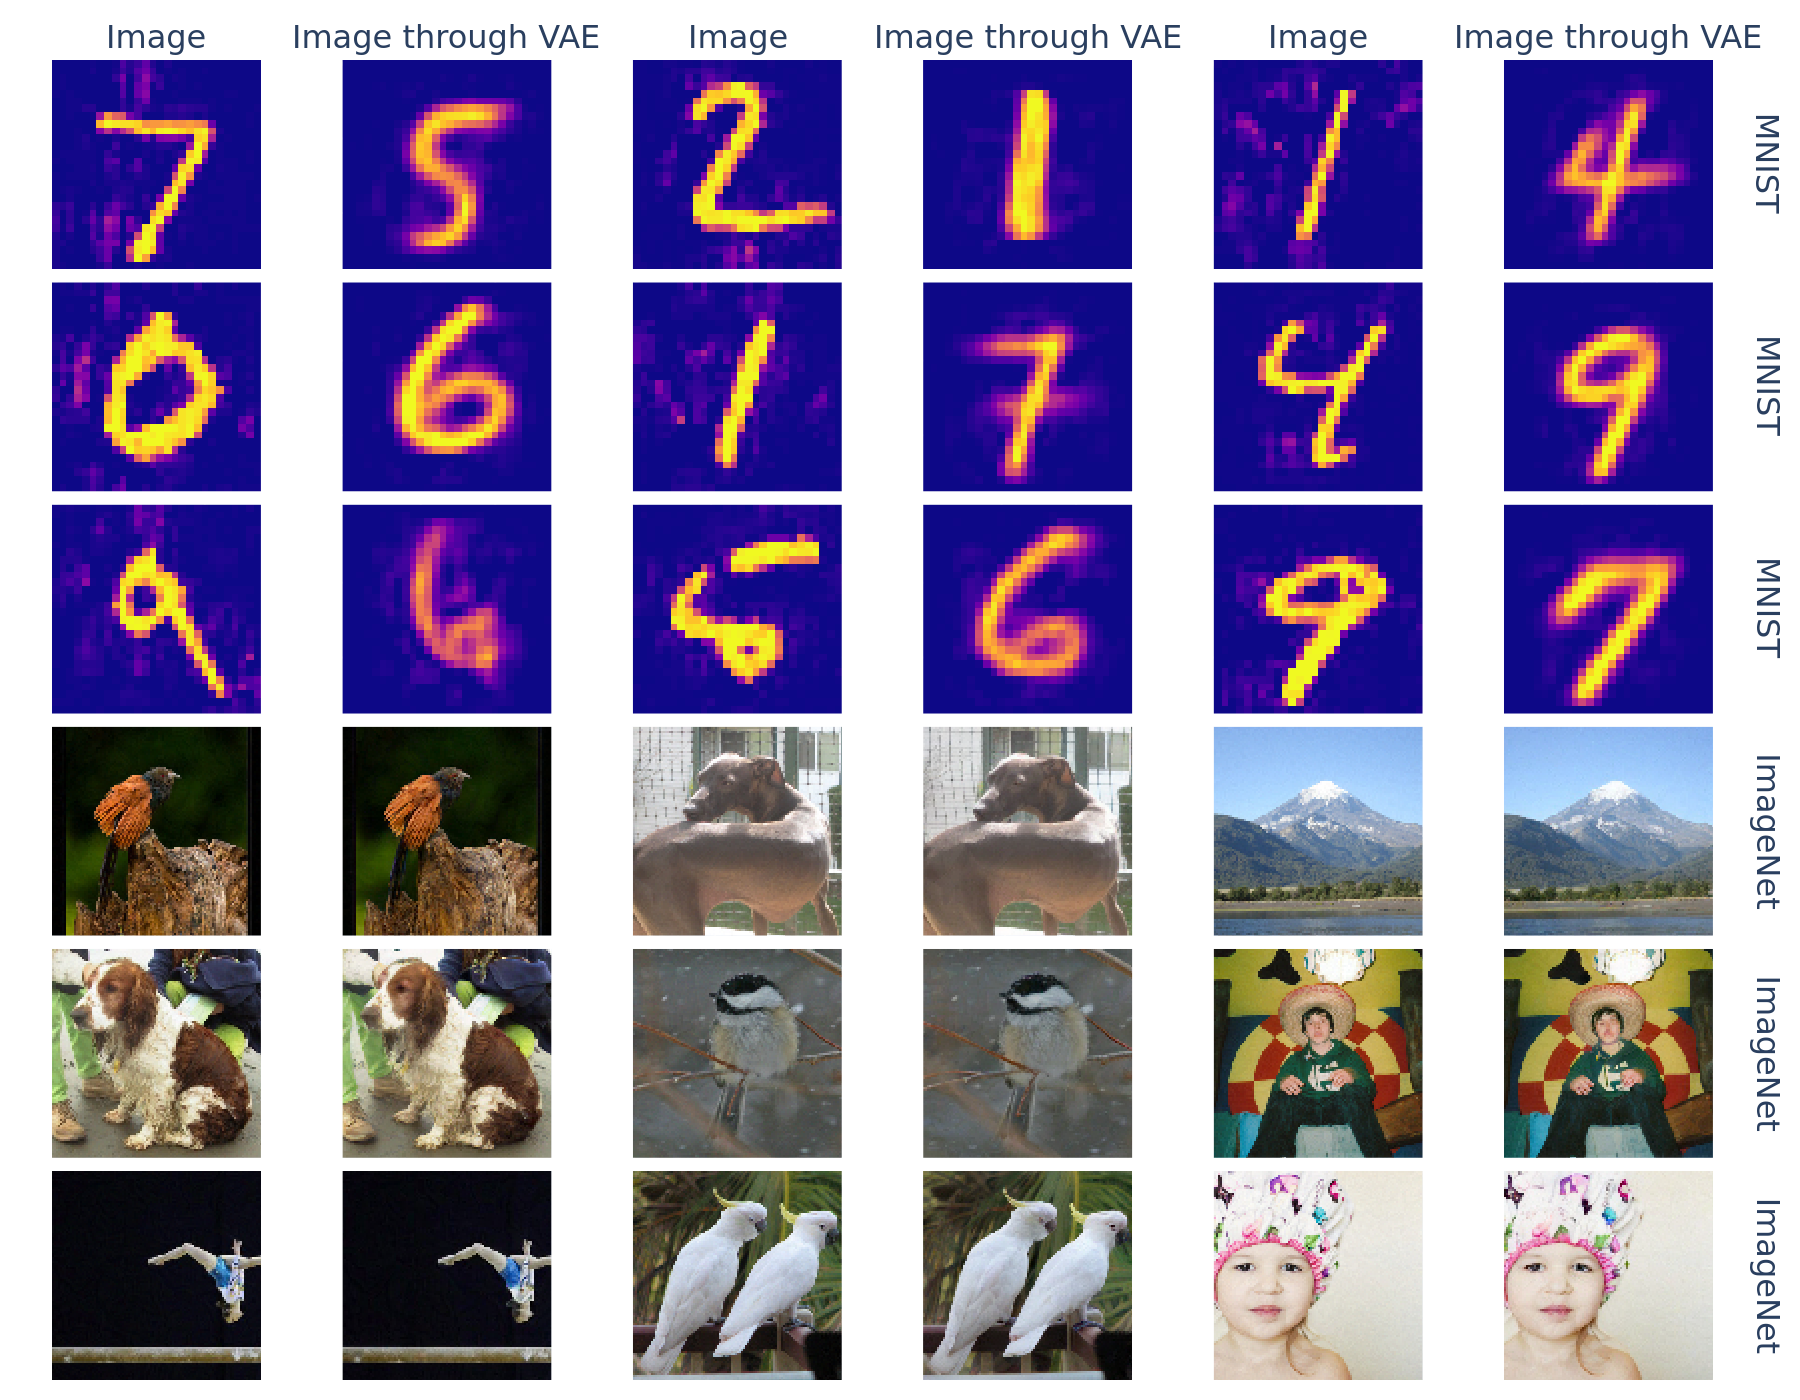
\includegraphics[width=0.9\textwidth]{../images/ae_many_attack_examples.png}
  \caption{
    Examples of iterated FGSM attacks through the autoencoder and classifier.
    \emph{Even columns:} Adversarial images.
    \emph{Odd columns:} The image on the left passed through the autoencoder.
  }
  \label{fig:ae_attack_examples_many}
\end{figure}

\paragraph{Can the MNSIT autoencoder produce an adversarial image?}
Probably not.
The attack on MNSIT seems to always either not work or produce
a different image through the VAE. One could try to make the autoencoder
output and adversarial perturbation by adding a term to the reconstruction
loss of the autoencoder. This would encourage the autoencoder to produce
an image that is close to its input.
However, I could not make this work, even when allowing the perturbation
arbitrarily large. Some options that I did not try are using different schedules for
the loss components or using attack methods not mentioned in this report.

The other question left is whether the ImageNet autoencoder can produce
and image that is completely different from the input.

% \clearpage
\subsection{Attacking the ImageNet autoencoder}

\begin{figure}[h]
  \centering
  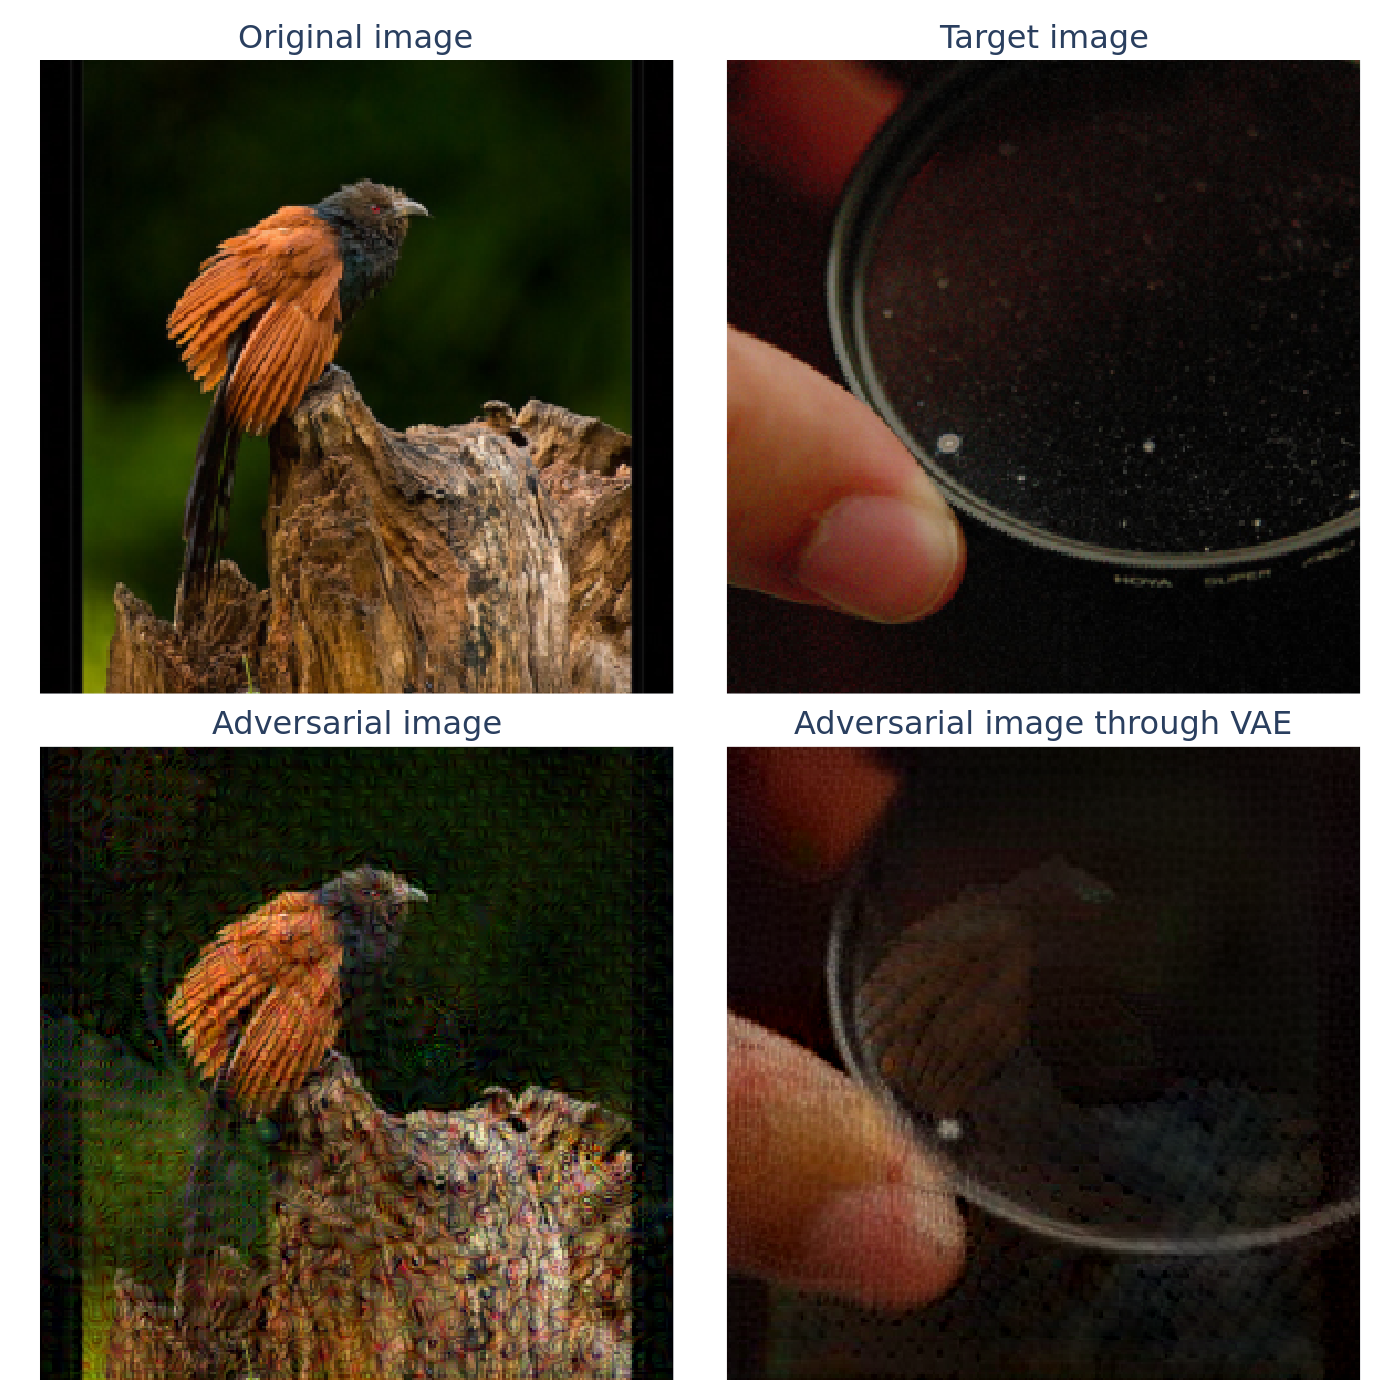
\includegraphics[width=0.6\textwidth]{../images/ae_targeted_attack_example.png}
  \caption{
    An example of a targeted attack that producing a different image
    through the autoencoder.
    The output image is almost correctly classified by the ResNet50,
    with 41\,\% "strainer" and "10\,\% "Petri dish" (the correct one).
  }
  \label{fig:ae_targeted_attack_example}
\end{figure}

I set out to attack the ImageNet autoencoder
so that it produces an image that is completely different from the input.
This was not an easy task, but is possible with a few tricks and caveats:
\begin{itemize}
  \item One needs to accept that the attack is quite visible on the image,
    as it seems to be impossible to do with $\e \leq 30 / 255$.
  \item The target image should not be too distant from the input image,
    and it is very helpful to pick a target image among the closest neighbours
    in norm $l_1$ or $l_2$ in the dataset.
  \item Using a loss that is a composite of different terms was the most helpful:
    \begin{enumerate}
      \item The reconstruction loss towards the target is of course necessary.
      \item A penalty for the $l_2$ norm of the perturbation helps to keep the
        perturbation small and prevent too much clamping to keep the perturbation
        in the valid range. A penalty of $0.1$ times the mean squared error was used
        everywhere in this report. It seems to be possible to train the attacks faster by
        starting with no penalty and then increasing it, but it is more hazardous.
      \item An attack with a lower norm (lower \e) is easier to get by setting \e high at first,
        then lowering it.
    \end{enumerate}
  \item The fact that the autoencoder is a VAE, and thus stochastic did not seem to
    play an important role in the attack, even though it was for getting FGSM to work on
    the smaller tasks.
\end{itemize}

\begin{figure}[h]
  \centering
  \includegraphics[width=0.9\textwidth]{../images/ae_many_targeted_attack_examples_ImageNet.png}
  \caption{
    Examples of attacks through the autoencoder.
    \emph{Even columns:} Adversarial images.
    \emph{Odd columns:} The image on the left passed through the autoencoder.
  }
  \label{fig:ae_targeted_attack_example2}
\end{figure}


\paragraph{Technical details}
The attacks seen in \autoref{fig:ae_targeted_attack_example} and
\ref{fig:ae_targeted_attack_example2}
 are all iterated FGSM attacks,
produced with 3 steps with different hyperparameters:
% \begin{itemize}
%   \item 600 iterations, $\e = 80 / 255$, $\text{l2\_penalty} = 0.1$, $lr = 0.04$
%   \item 300 iterations, $\e = 80 / 255$, $\text{l2\_penalty} = 0.5$, $lr = 0.01$
%   \item 200 iterations, $\e = 80 / 255$, $\text{l2\_penalty} = 1.0$, $lr = 0.004$
% \end{itemize}
% As table instead:
\begin{center}
  \begin{tabular}{llll}
    Iterations & $\e$ & L2 Penalty & Learning rate \\
    \hline
    600 & $70 / 255$ & $1.0$ & $0.004$ \\
    300 & $70 / 255$ & $1.0$ & $0.001$ \\
    200 & $70 / 255$ & $1.0$ & $0.0004$ \\
  \end{tabular}
\end{center}


\begin{remark}
  Attacking an autoencoder to produce a different image, can be detected
  very easily, by checking if the reconstruction loss is high.
  This seems to be a good sanity check to have in place when using
  an autoencoder as a defence mechanism.
\end{remark}

\clearpage
\section{Norm detection}

Seeing the attacks that produce a completely different image
through the autoencoder, I was reminded of chaos theory,
as we have a small perturbation of the input that produces
large changes in the output.
I wondered if there was a nicely defined Lyapunov exponent
that applied to this system or maybe to many neural networks.

The first I checked was the evolution of the distance in
activation space between the original image and the adversarial image,
at each layer of the network, expecting to see where in
the networks the perturbation was amplified. Do they smoothly
separate over time, or is there a specific (set of) layer(s)
where the perturbation is amplified?

\begin{figure}[h]
  \centering
  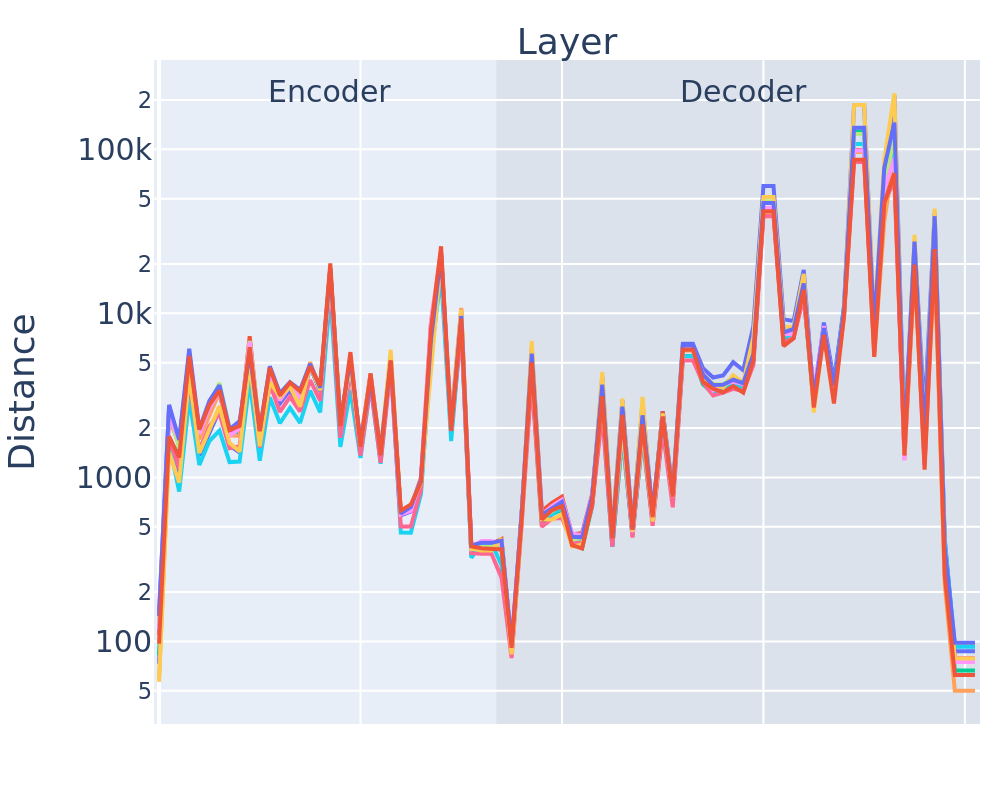
\includegraphics[width=0.6\textwidth]{../images/ae_attack_distances.png}
  \caption{
    Distance in activation space between the original image and the adversarial image
    at each layer of the autoencoder, for the 12 attacks from
    \autoref{fig:ae_attack_examples_many}.
  }
  \label{fig:ae_attack_distances}
\end{figure}

Well, if one thing is clear, it's that it's not clear on \autoref{fig:ae_attack_distances}.
Indeed, the norm of the activations varies by several orders of magnitude
between layers and mediates strongly the distance between the activations.
It might be surprising at first that the norms go as high as $200\,000$,
but the size of those tensors also reaches 16 million elements.

\begin{figure}[H]
  \centering
  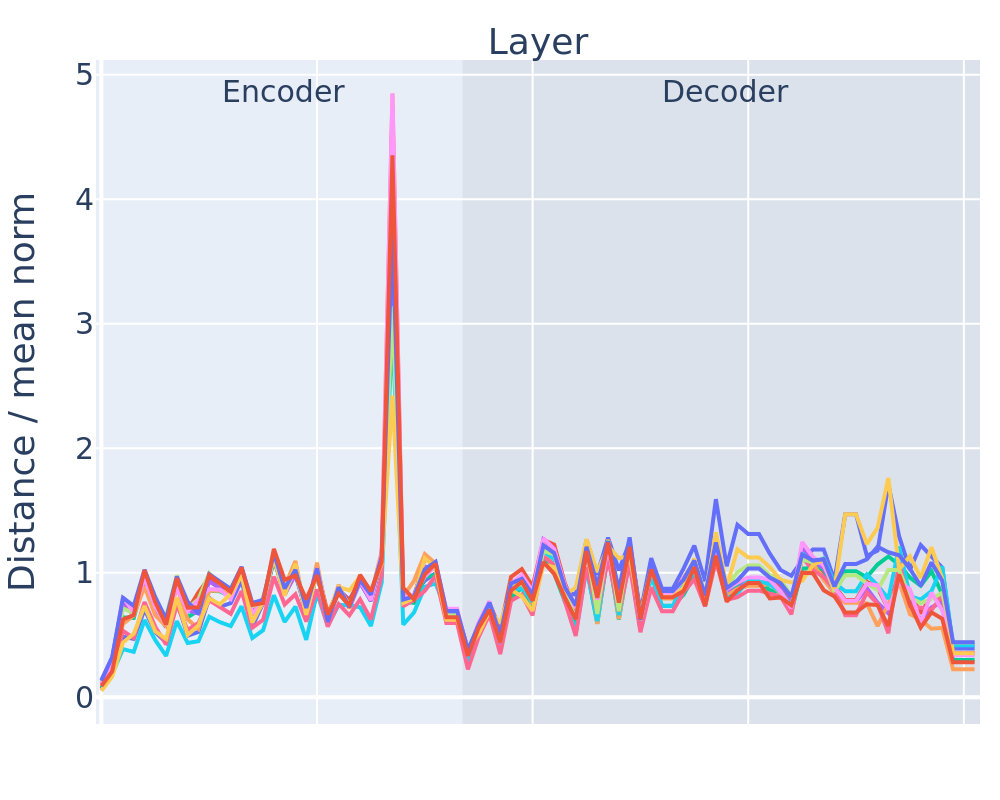
\includegraphics[width=0.8\textwidth]{../images/ae_attack_distances_normalized.png}
  \caption{
    Distance in activation space between the original image and the adversarial image
    at each layer of the autoencoder, for the 12 attacks from
    \autoref{fig:ae_attack_examples_many}.
    The distance is normalised by the average activation norm of 100 images
    from the test dataset.
  }
  \label{fig:ae_attack_distances_normalized}
\end{figure}

Surprisingly, when normalising, we have a very clear spike at the end of the encoder.
This spike is present in every of the 12 attacks.
And corresponds to the output of the attention, before normalisation
and before the last three convolutions of the encoder.

I first tried to understand why the distance between the clean
and corrupt activations was so high, do they have a different norm?
Or is it because the activations are in different directions?

\begin{figure}[h]
  \centering
  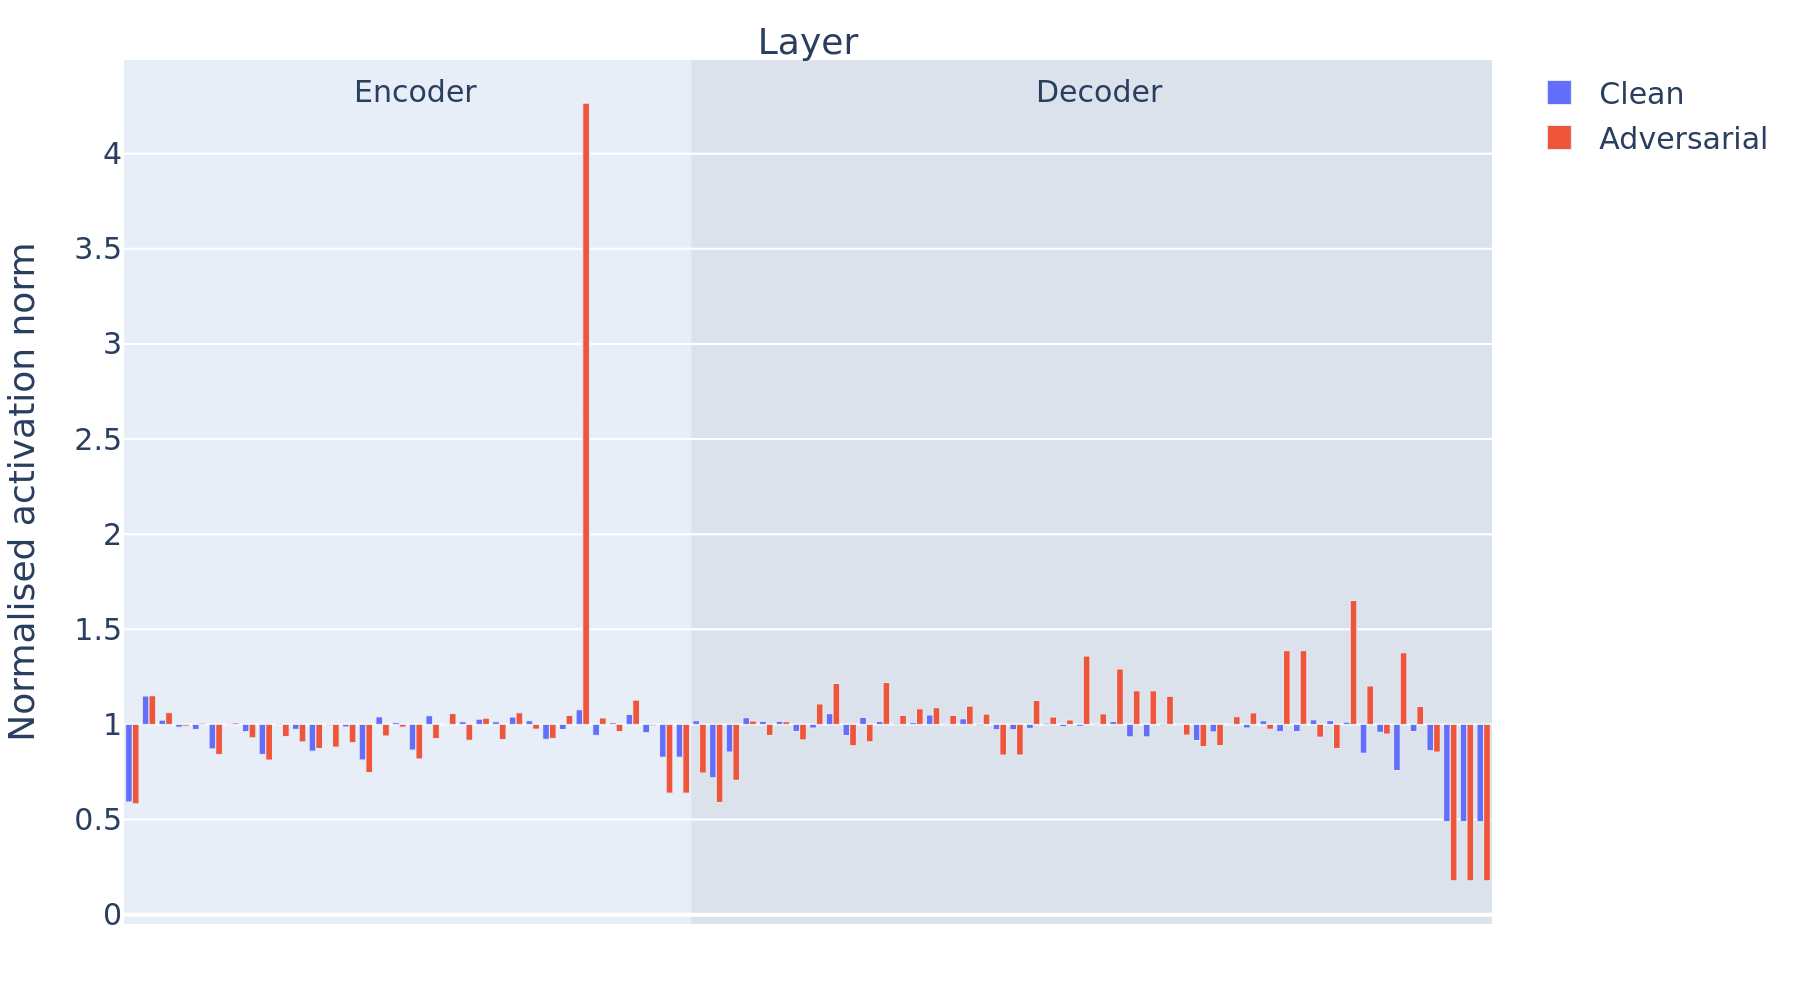
\includegraphics[width=0.9\textwidth]{../images/ae_activation_norm.png}
  \caption{
    Layer-by-layer plot of the norm of the activations of the autoencoder,
    normalised by the average norm of 100 images from the dataset.
  }
  \label{fig:ae_activation_norm}
\end{figure}

Looking at the norms in \autoref{fig:ae_activation_norm} reveals
even more clearly, a single layer where the norm of the activations is about
4 times larger than the average norm of the dataset.
There is also much more variance in the norm of activations
on adversarial images than on clean images, whose blue
bars can barely be seen in the plot.

This gives a straightforward way to detect this kind of adversarial
attacks: pass the image through the autoencoder and check if the
norm of the activations at this layer is larger than usual.


\begin{remark}
  It is still more straightforward to check the reconstruction loss.
\end{remark}

\subsection{Generalisation}

The last question is whether this phenomenon is specific to
our setup, or is a more general phenomenon.

\paragraph{Different autoencoders}
I tried the same experiment on the MNIST autoencoder
whose results are shown in
\autoref{fig:ae_activation_norm_mnist}
but could not get a good autoencoder running on CIFAR10.
On MNIST, there is no clear spike and the norms of adversarial
activations are even a little bit smaller than the norms of clean activations.
However, this is an artefact of the choice of the attacks to plot,
and other attacks did not show this pattern.

Overall, this suggests that the phenomenon is either specific
to StabilityAI's autoencoder, or to larger autoencoders.

\begin{figure}[h]
  \centering
  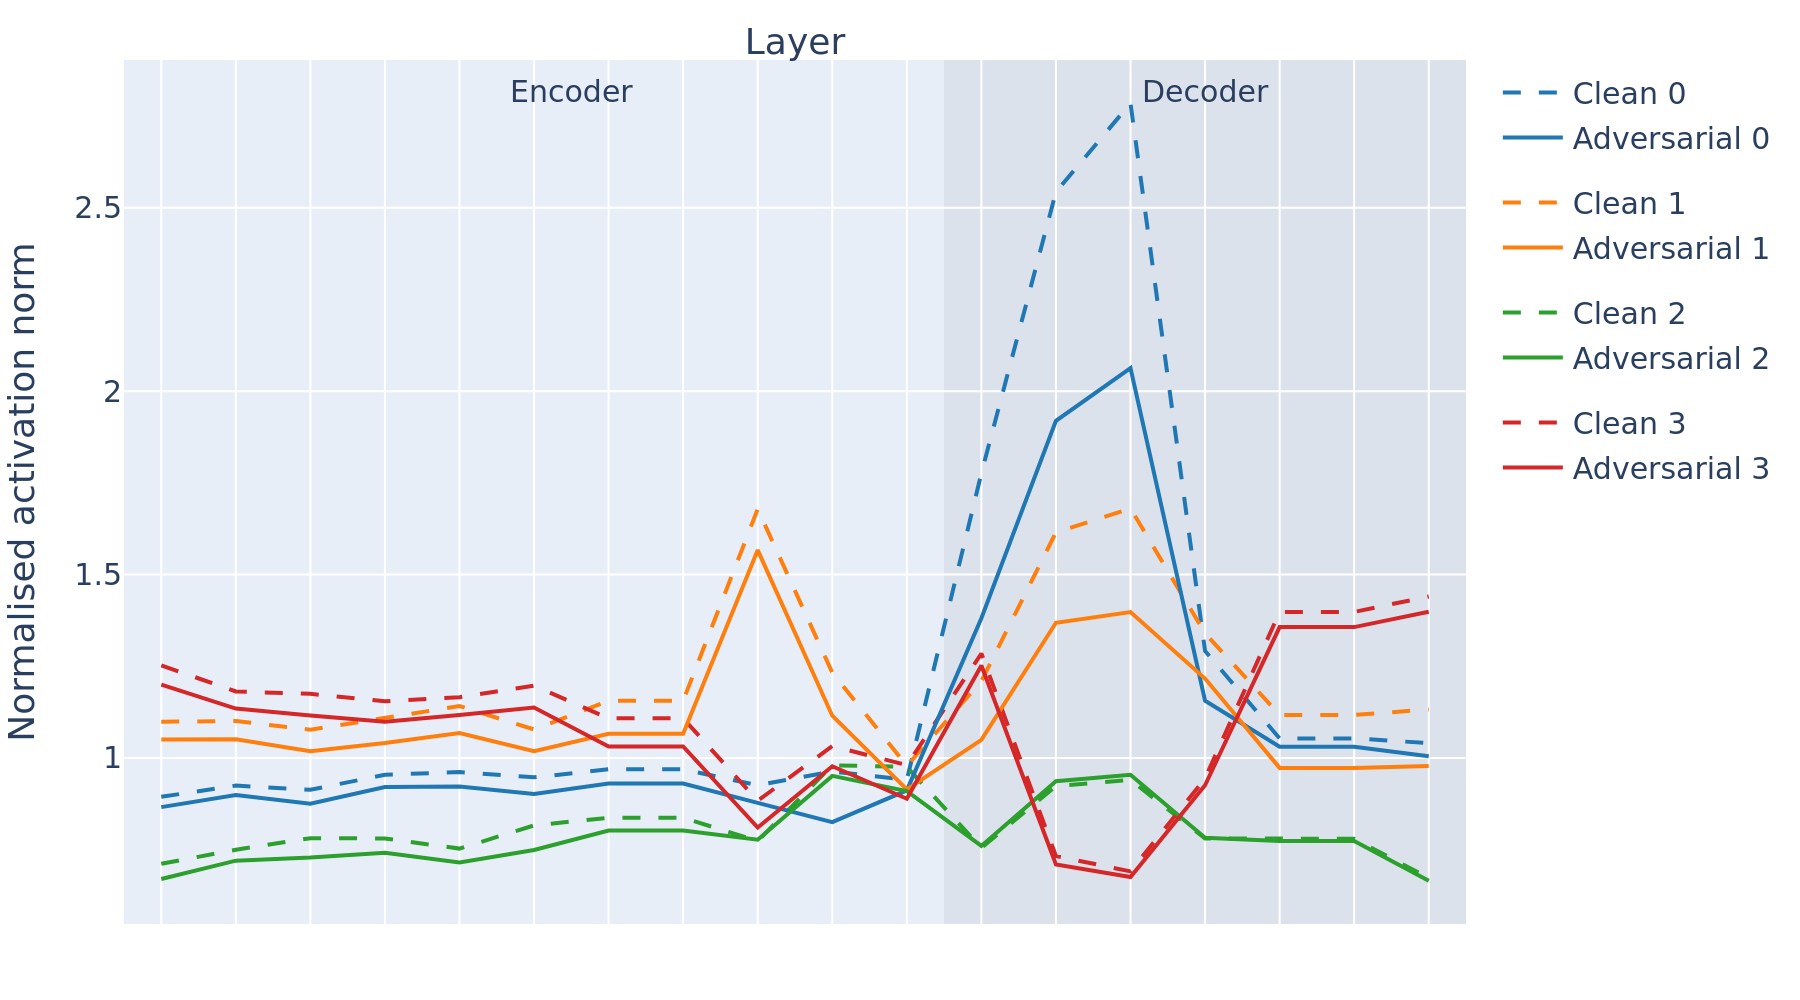
\includegraphics[width=0.9\textwidth]{../images/ae_activation_norm_MNIST.png}
  \caption{
    Layer-by-layer plot of the norm of the activations of the autoencoder,
    normalised by the average norm of 100 images from the dataset.
  }
  \label{fig:ae_activation_norm_mnist}
\end{figure}


Similarly, attacking only the classifier, without the autoencoder,
does not produce this pattern.

\clearpage
\section*{Bonus}
\addcontentsline{toc}{section}{Bonus}

As a bonus, we show a few images that produce interesting results when
passed through the autoencoder.

\begin{figure}[h]
  \centering
  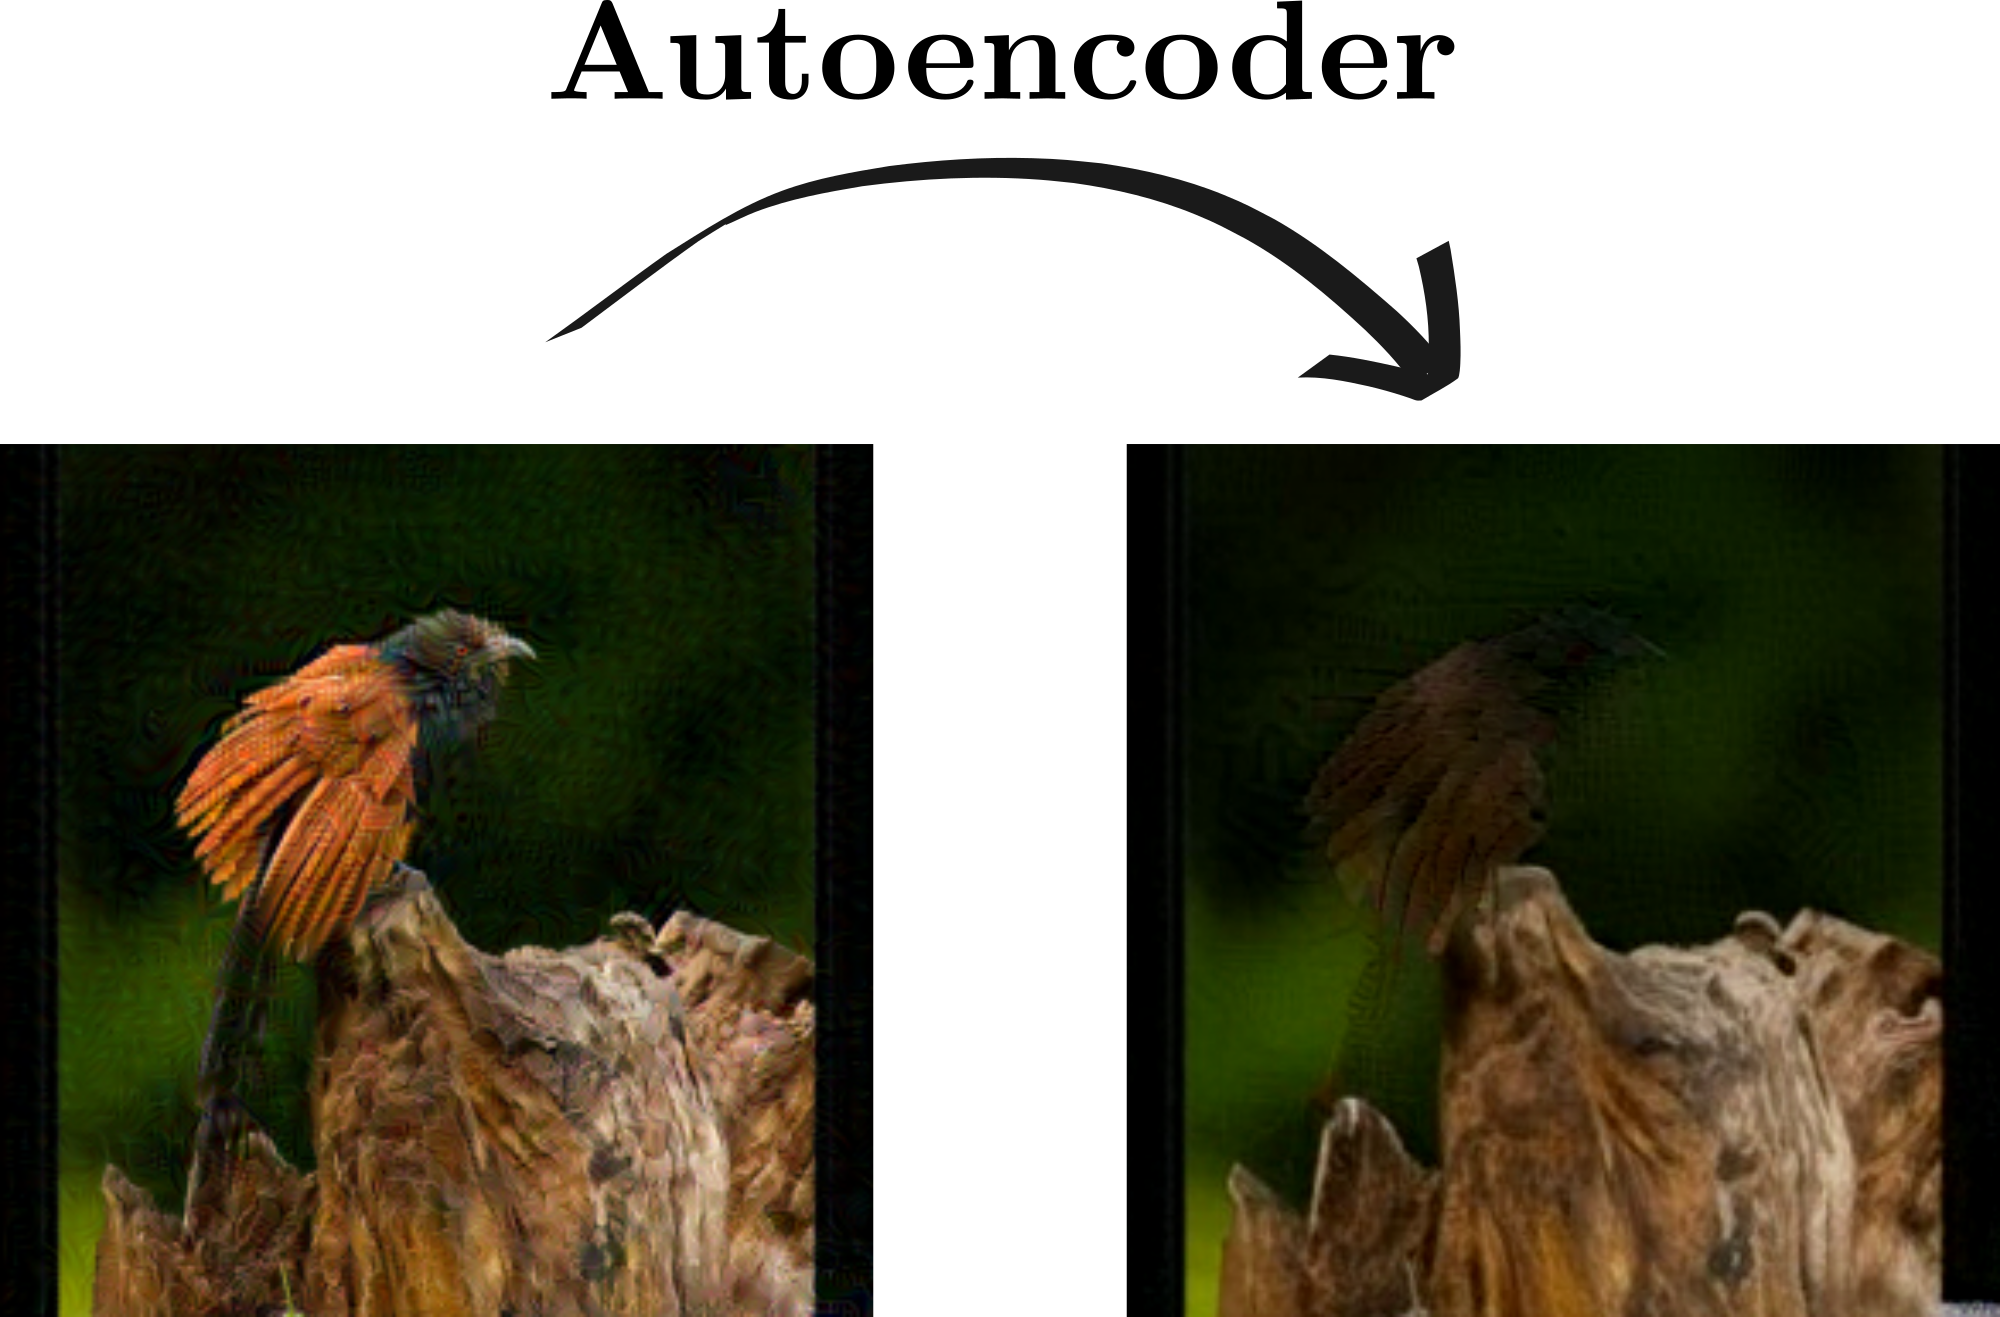
\includegraphics[width=0.8\textwidth]{../images/bird-no-bird.png}
  \caption{
    A bird with an invisibility cloak.
    It is easier to attack when only a part of the image is changed,
    as the two are more similar.
  }
\end{figure}

Note that making birds disappear is something humans have been really good at,
without the help of neural networks.
60\% of European land birds have disappeared between 1980 and 2016
\cite{Rigal2023FarmlandPA}, for a total of 800 million birds.

However, making a bird appear out of thin air is something that
only the best of magicians have been able to do.

\begin{figure}[h]
  \centering
  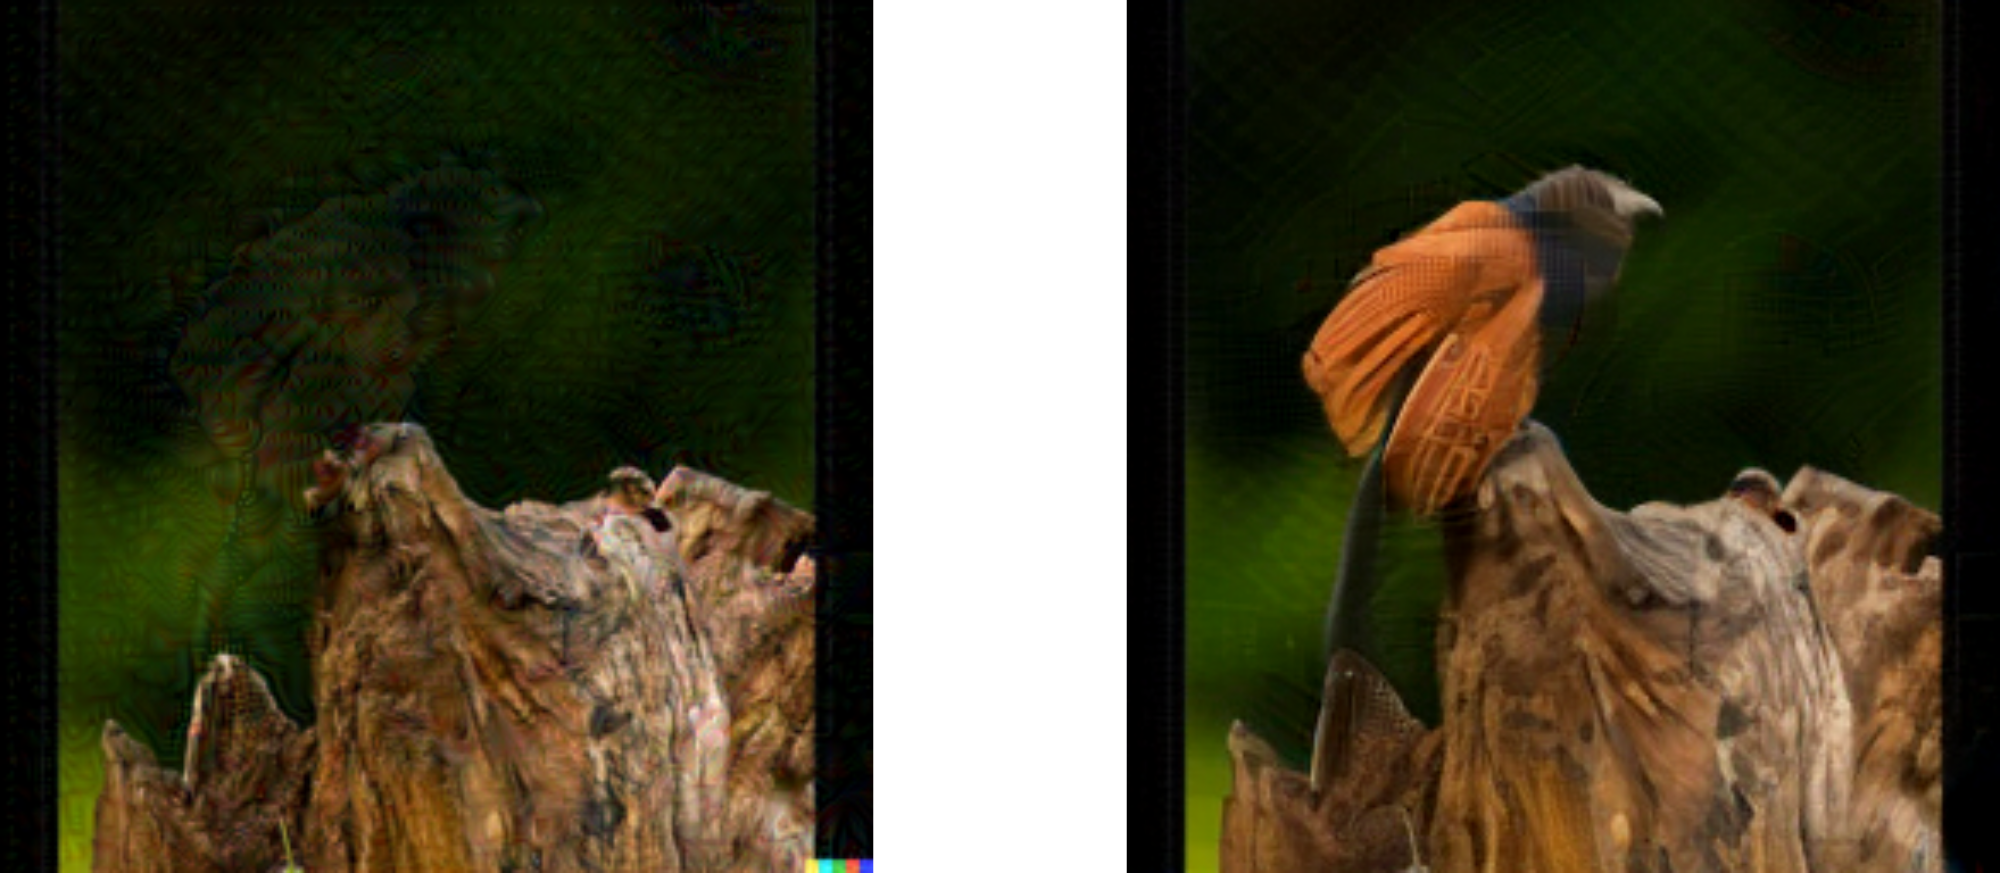
\includegraphics[width=0.8\textwidth]{../images/bird-resurected.png}
  \caption{
    A bird appears out of thin air.
  }
\end{figure}





% \section*{Conclusion}
% \addcontentsline{toc}{section}{Conclusion}


\clearpage
% \nocite{*}
\addcontentsline{toc}{section}{Bibliography}
\bibliographystyle{apalike}
\bibliography{bibliography.bib}

\end{document}
